\documentclass{sp}\usepackage[]{graphicx}\usepackage[]{color}
%% maxwidth is the original width if it is less than linewidth
%% otherwise use linewidth (to make sure the graphics do not exceed the margin)
\makeatletter
\def\maxwidth{ %
  \ifdim\Gin@nat@width>\linewidth
    \linewidth
  \else
    \Gin@nat@width
  \fi
}
\makeatother

\definecolor{fgcolor}{rgb}{0.345, 0.345, 0.345}
\newcommand{\hlnum}[1]{\textcolor[rgb]{0.686,0.059,0.569}{#1}}%
\newcommand{\hlstr}[1]{\textcolor[rgb]{0.192,0.494,0.8}{#1}}%
\newcommand{\hlcom}[1]{\textcolor[rgb]{0.678,0.584,0.686}{\textit{#1}}}%
\newcommand{\hlopt}[1]{\textcolor[rgb]{0,0,0}{#1}}%
\newcommand{\hlstd}[1]{\textcolor[rgb]{0.345,0.345,0.345}{#1}}%
\newcommand{\hlkwa}[1]{\textcolor[rgb]{0.161,0.373,0.58}{\textbf{#1}}}%
\newcommand{\hlkwb}[1]{\textcolor[rgb]{0.69,0.353,0.396}{#1}}%
\newcommand{\hlkwc}[1]{\textcolor[rgb]{0.333,0.667,0.333}{#1}}%
\newcommand{\hlkwd}[1]{\textcolor[rgb]{0.737,0.353,0.396}{\textbf{#1}}}%
\let\hlipl\hlkwb

\usepackage{framed}
\makeatletter
\newenvironment{kframe}{%
 \def\at@end@of@kframe{}%
 \ifinner\ifhmode%
  \def\at@end@of@kframe{\end{minipage}}%
  \begin{minipage}{\columnwidth}%
 \fi\fi%
 \def\FrameCommand##1{\hskip\@totalleftmargin \hskip-\fboxsep
 \colorbox{shadecolor}{##1}\hskip-\fboxsep
     % There is no \\@totalrightmargin, so:
     \hskip-\linewidth \hskip-\@totalleftmargin \hskip\columnwidth}%
 \MakeFramed {\advance\hsize-\width
   \@totalleftmargin\z@ \linewidth\hsize
   \@setminipage}}%
 {\par\unskip\endMakeFramed%
 \at@end@of@kframe}
\makeatother

\definecolor{shadecolor}{rgb}{.97, .97, .97}
\definecolor{messagecolor}{rgb}{0, 0, 0}
\definecolor{warningcolor}{rgb}{1, 0, 1}
\definecolor{errorcolor}{rgb}{1, 0, 0}
\newenvironment{knitrout}{}{} % an empty environment to be redefined in TeX

\usepackage{alltt}
\usepackage{linguex}
\usepackage{changepage}
\usepackage{float}
\usepackage{booktabs}
\usepackage{subscript}
\usepackage{subfiles}
\usepackage{subfigure}
\usepackage{tabularx}
\usepackage{csquotes}
\usepackage{soul}
\usepackage{multirow}
\usepackage{multicol}
\usepackage{placeins}
\usepackage{longtable}

\newcommand{\dobib}{\bibliography{prag}}

\setstcolor{red}

\newcommand{\flag}[1]{\textcolor{red}{\bf #1}}
\newcommand{\iflag}[1]{#1}
\newcommand{\ignore}[1]{}
\newenvironment{myenv}{\begin{adjustwidth}{1cm}{}}{\end{adjustwidth}}
\newcommand{\change}[1]{\textcolor{green}{\bf #1}}
\newcommand{\revised}[1]{\textcolor{blue}{#1}}
\pdfauthor{Ekaterina Kravtchenko and Vera Demberg}
\pdftitle{Informationally Redundant Event Descriptions Alter Prior Beliefs about Event Typicality}
\pdfkeywords{Psycholinguistics; redundancy; context-dependent implicatures; accommodation}

\title[]{Informationally Redundant Utterances Alter Prior Beliefs about Event Typicality
}

\author[]{}
\IfFileExists{upquote.sty}{\usepackage{upquote}}{}
\begin{document}



\renewcommand{\dobib}{}

\maketitle

\begin{abstract}
Most theories of pragmatics and language processing predict that speakers avoid excessive informational redundancy. Informationally redundant utterances are, however, quite common in natural dialog. From a comprehension standpoint, it remains unclear how comprehenders interpret these utterances, and whether they make attempts to reconcile the `dips' in informational utility with expectations of `appropriate' or `rational' speaker informativity. We show that informationally redundant (overinformative) utterances can trigger pragmatic inferences that increase utterance utility in line with comprehender expectations. In a series of 3 studies, we look at utterances which refer to stereotyped event sequences describing common activities (\emph{scripts}). When comprehenders encounter utterances describing events that can be easily inferred from prior context, they interpret them as signifying that the event conveys new, unstated information (i.e.~an event otherwise assumed to be habitual, such as \emph{paying the cashier} when \emph{shopping}, is reinterpreted as non-habitual). Further, we show that the degree to which such inferences are triggered depends on the framing of the utterance. In the absence of prosodic or discourse markers indicating the speaker's specific intent to communicate the given information, such inferences are far less likely to arise. Overall, the results demonstrate that excessive conceptual redundancy leads to comprehenders revising the conversational common ground, in an effort to accommodate unexpected dips in informational utility.
\end{abstract}

\begin{keywords}
  experimental pragmatics; redundancy; psycholinguistics; context-dependent implicatures; accommodation; overinformativeness; prosody.
\end{keywords}

\pagebreak

\tableofcontents

\pagebreak

\listoftables

\pagebreak

\listoffigures

\pagebreak

\section{Introduction}\label{intro}

\subfile{sections/intro.tex}

\section{Related Work}\label{related-work}

\subfile{sections/related.tex}

\section{Experimental Procedure}\label{expintro}

\subfile{sections/expintro.tex}

\section{Experiment 1: Implicit Prosodic Emphasis}\label{exp1}



We first test whether informationally redundant event descriptions trigger \textit{non-habituality} inferences when the utterance is apparently effortful, intentional, and attentionally prominent -- here signalled by an exclamation mark at the end of the utterance (this would disprove the "no inference" hypothesis). Intuitively, exclamatory intonation is a natural way of introducing something that may be noteworthy or unusual \citep{Rett2011}, without otherwise altering the semantic content of the utterance. When inferences are context-dependent \citep[and even if they are not; see][]{Degen2015b}, speakers generally provide multiple signals of their intended meaning, in order to make the inferences easier to compute for the comprehender. One would expect this to particularly be the case when the meaning of the utterance substantially violates expectations or previously held beliefs, as opposed to simply providing new but marginally expected (or at least unsurprising) information.

We present naive participants with a limited number of brief `narratives,' which set up the common ground context, relationships between discourse participants, and some typical or atypical properties of their usual behavior (where relevant). Some of the narratives include brief dialogue between two discourse participants at the end (which may include informationally redundant or non-redundant event descriptions). After reading the narratives, participants rate how habitual they believe certain behaviors in the story to be. We expect participants who read informationally redundant event descriptions to infer that the utterance in fact signals that the event is relatively unexpected, or non-habitual (as only relatively unexpected events warrant explicit mention). In contrast, those participants who read non-redundant event descriptions should draw no such inferences.

\subsection{Methods}

\subsubsection{Participants}

700 eligible participants (%
760
 total; median age bracket %
26-35
; %
50
\% female), were recruited on Amazon Mechanical Turk. The task was open only to workers located in the US, and with an approval rating of $\geq$ 95\%. All workers were asked to state their native childhood language (with no penalty for stating a language other than English, to encourage accurate reporting), age bracket (under 18, 18-25, 26-25, and up, in intervals of 10), and gender.  Those who did not indicate English, or listed their age as outside the interval of 18-65, were excluded from all analysis (%
60
; %
7.89
\%), with additional participants recruited to replace them.

Those who did not provide accurate or plausible responses to the trial questions, all of which had a range of `valid' and `invalid' responses, were unable to proceed to the main task, and their data as a result was not recorded by the platform (e.g., those who rated the likelihood of 50\% heads on multiple fair coin flips as low, compared to other possible outcomes)\footnote{Since this data was not recorded, we cannot report on the number of participants who were unable to proceed to the main task.}. Participants were likewise unable to proceed in the study, or submit their results, without having answered all questions.

\subsubsection{Design}

The primary question of interest is whether informationally redundant utterances (in this case, descriptions of highly \textit{habitual} activities) are perceived as potentially violating conversational norms at face value, and whether they consequently trigger pragmatic inferences. These inferences should lead to the revision of common-ground beliefs about the \textit{habituality} of said activities (and so `repair' the violation, or dip in informational utility): 

\ex. "John just came back from the grocery store. \textbf{He paid the cashier!}"

The bolded utterance here, given a `default' or \textit{ordinary} common ground, is \textbf{\textit{informationally redundant}}.  We hypothesize that readers will infer that \textit{John} does \textit{not} habitually pay the cashier, as such a scenario would justify overt mention of \textit{John's} cashier-paying. The informational redundancy arises due to the high \textit{conceptual} (or \textit{event}) \textit{predictability} of \textit{paying the cashier}, and is resolved if one assumes that this activity is not as habitual, or predictable as initially assumed. 

We also wanted to see whether the inference (that an activity is less habitual than would otherwise be expected) could be cancelled by manipulating the common ground.

\paragraph{Common ground manipulation}

The activity described becomes `non-habitual' given a \textit{wonky} common ground\footnote{We borrow the term \textit{wonky} from \citet{Degen2015a}, where it is similarly used to describe non-default common grounds, in which typical rules as to how things proceed are expected to not hold, and which comprehenders may assume when encountering otherwise pragmatically infelicitous utterances.} such as in \ref{shoplifter}, where the context suggests that typical assumptions (e.g., that some given individual would \textit{pay the cashier} when they \textit{go to the grocery store}) may not hold.  At that point, the activity description ceases to be informationally redundant, and the inference should therefore not arise. This control condition keeps the description itself constant and manipulates only the common ground. It thus ensures that any effect we measure is in fact due to the presence of informational redundancy, and verifies that comprehenders are sensitive to discourse context.

\ex.\label{shoplifter} \textsc{Common Ground Context}: John habitually doesn't pay.  
``John just came back from the grocery store.  \textbf{He paid the cashier!}"

Finally, we wanted to provide a baseline for `typical' interpretation of non-redundant event descriptions; and to confirm that similarly structured descriptions of conventionally \textit{non-habitual} activities, as in \ref{apples}, do not provoke similar inferences (which would suggest a problem with the stimulus design or response measure). In \ref{apples}, the utterance is not informationally redundant, and is not expected to generate any specific inferences. We also wanted to confirm that the \textit{wonky} common ground in the previous example does not significantly affect the interpretation of conventionally \textit{non-habitual} event mentions (which would suggest that there is an unexpected effect of context manipulation on stimulus interpretation, in general): 

\ex.\label{apples} \textsc{Context}: \textit{Ordinary} \textbf{or} John habitually doesn't pay.  
``John just came back from the grocery store.  \textbf{He got some apples!}"

As in \ref{shoplifter}, participants should draw no non-habituality inferences here, as the event described is not (typically) overly habitual. These conditions therefore provide a secondary control measure.

\subsubsection{Materials}

24 stimuli were constructed as brief stories/narratives, based on distinct stereotyped scripts or events. Each story had one of 2 context types (\textit{ordinary} vs. \textit{wonky} common ground, relative to the \textit{conventionally habitual} script activity). In all stories, declarative utterances, spoken by one of the discourse participants, described one of 2 types of script activities (\textit{conventionally habitual} vs. \textit{non-habitual}), making a total of 4 conditions\footnote{The complete list of stimuli can be found in our online repository: \url{https://osf.io/h5afr/?view_only=ff5859d3f33b485d95254395f95a52dc}}.

\textit{Conventionally habitual} activities \ref{ex:habitual1} can normally be inferred simply from the `speaker' having invoked the script, while \textit{non-habitual} activities \ref{ex:nonhabitual1} can not be inferred automatically, as they may only occasionally occur as part of the script activity. To clarify, we are using the term \textit{conventionally habitual} to specify that the event almost invariably occurs as part of the event script (under normal conditions, and for typical individuals). Initial common ground was either \textit{ordinary} ([1a] below) with respect to the script, or \textit{wonky}, in that it implied the \textit{conventionally habitual} event was in fact unusual for the event participant ([1b] below): 

\ex.\label{ex:habitual1} \centering\textsc{Conventionally Habitual Event}
\vspace{-0.1cm}
\centering

\begin{longtable}{p{0.435\textwidth}|p{0.435\textwidth}}
$[$1a$]$ John \textbf{often goes to the grocery store around the corner from his apartment\textsubscript{ordinary}} & $[$1b$]$ John \textbf{is typically broke, and doesn't usually pay when he goes to the grocery store\textsubscript{wonky}}          \\
\hline
\multicolumn{2}{p{0.9\textwidth}}{$[$2$]$ Recently, he came home from the store with groceries.  When he came in, he saw his roommate Susan in the hallway, and started talking to her about his trip to the store.  As he went to the kitchen to put his groceries away, Susan went to the living room, where their roommate Peter was watching TV.} \\
\hline
\multicolumn{2}{p{0.9\textwidth}}{$[$3$]$ Susan said to Peter: ``John just came back from the grocery store. $[$4$]$ He \textbf{paid the \mbox{cashier\textsubscript{habitual}}}!''}
\end{longtable}
\addtocounter{table}{-1}

The context/common ground manipulation in [1b] was used in order to render the \textit{conventionally habitual} event unusual, or at least not habitual. Conventionally \textit{non-habitual} activities could not be automatically inferred from the script having been invoked: 

\ex.\label{ex:nonhabitual1} \centering\textsc{Non-habitual Event}
\vspace{-0.1cm}
\centering

\begin{longtable}{p{0.435\textwidth}|p{0.435\textwidth}}
$[$1a$]$ John \textbf{often goes to the grocery store around the corner from his apartment\textsubscript{ordinary}} & $[$1b$]$ John \textbf{is typically broke, and doesn't usually pay when he goes to the grocery store\textsubscript{wonky}}          \\
\hline
\multicolumn{2}{p{0.9\textwidth}}{$[$2$]$ Recently, he came home from the store with groceries.  When he came in, he saw his roommate Susan in the hallway, and started talking to her about his trip to the store.  As he went to the kitchen to put his groceries away, Susan went to the living room, where their roommate Peter was watching TV.} \\
\hline
\multicolumn{2}{p{0.9\textwidth}}{$[$3$]$ Susan said to Peter: ``John just came back from the grocery store. $[$4$]$ He \textbf{got some \mbox{apples\textsubscript{non-habitual}}}!''}
\end{longtable}
\addtocounter{table}{-1}

Participants saw either only the common ground \textit{context} [1] and \textit{discourse setup} [2] (without numbering or special formatting), which enabled us to collect estimates of how habitual activities are believed to be, based on the context alone (\textit{pre-utterance beliefs}); or the entire text, which enabled us to collect estimates of how habitual activities are believed to be, based on both the context \textit{and} the event description [4] (\textit{post-utterance beliefs}). 

Following each passage, participants were queried as to how habitual they believed the \textit{conventionally habitual} and \textit{non-habitual} activities (as well as 2 other scenario-relevant distractor activities) were, for the person who was the subject of the discourse (the individual mentioned in the context [1] and event description [4]):

1. How often do you think John usually \textit{pays the cashier}, when going shopping?
2. How often do you think John usually \textit{gets apples}, when going shopping?
3. How often do you think John usually goes to the grocery store?
4. How often do you think Susan and Peter usually talk to each other?

Each question could be responded to on a continuous sliding scale of `Never' to `Always' (see Fig. \ref{fig:slider}). The slider itself was not visible until the participant clicked on the point on the scale that they thought was most appropriate, to avoid having people default towards a particular value. After they responded to all questions, participants could submit their answers. Once they did, the next passage was displayed on a new screen. 

12 of the stimuli included 3 discourse participants -- one of whom engaged in the script activity (\textit{John}), the second who learned from that participant that they engaged in it (\textit{Susan}), and the third to whom the second communicated this fact (\textit{Peter}). The other 12 only included two -- the subject of the discourse, who engaged in the activity (\textit{John}), and the second participant to whom they communicated this fact (\textit{Susan}). Compared to the example above, for instance, \textit{John} might instead be communicating directly to \textit{Susan}: ``\textit{I just got back from the grocery store. I paid the cashier!}". 

The construction of these stimuli was constrained in several ways. The scripts (e.g., \textit{going shopping}) needed to be sufficiently complex to include multiple subactivities or subroutines, and there needed to be habitual as well as non-habitual subactivities (\textit{paying the cashier}, \textit{getting apples}). It needed to be possible for the script to play out without the habitual activity having taken place -- otherwise, the discourse would be incoherent, or the inference would not be drawn.  For example, one arguably cannot play \textit{tennis} at all, without using a \textit{racket}. There was also established common ground between all discourse participants, so that all were plausibly (from the point of view of the reader) aware of the typical habits of the discourse subject, particularly with regard to the activity described. Finally, the activities needed to be sufficiently stereotyped and (relatively) culturally invariant, so that participants could be expected to agree on what a script entailed, which activities were or weren't obligatory to the script sequence, etc..

All stimuli were normed on 3 qualities (in separate tasks): whether the activity fell into the \textit{habitual} or \textit{non-habitual} activity bin; whether the common ground manipulation was effective; and whether participants found it plausible that the script could be engaged in without the \textit{habitual} activity.  For activity predictability norming, participants were asked to rate the habituality of the activity (on a 0-100 scale), with an arbitrary cutoff of 70 between activity types.  \textit{Non-habitual} activities were on average rated 48.0 (25.1-68.1), and \textit{habitual} activities were rated 87.8 (78.1-95.2).  For common ground norming, participants rated \textit{habitual} activities in \textit{ordinary} (mean 83.4 [72.2-96.9]) or \textit{wonky} common grounds (mean 39.2 [20.7-62.0]), with a within-item difference between the two of at least 15 points (mean difference 44.2; [19.8-72.9]); \textit{non-habitual} activities had to score below 70 regardless of common ground (mean 45.2; on average 10.7 points higher in the \textit{ordinary} common ground).  For plausibility norming, a statement in the form of `\textit{John \textbf{went shopping}, but didn't pay the cashier}' was rated as either \textit{coherent} (plausible) or \textit{incoherent} (implausible), with criteria being a majority of participants finding the statement coherent (\textit{habitual}: 91\% [67\%-100\%]; \textit{non-habitual}: 94\% [80\%-100\%]).

\subsubsection{Measures}

To measure comprehender beliefs regarding activity habituality, each story we presented was followed by 4 questions presented in random order, regarding activities mentioned in the story (including both conventionally \textit{habitual} and \textit{non-habitual} activities associated with the stimulus item). The questions were accompanied by sliding scales which ranged from \textit{Never} to \textit{Always}, where participants could select any point along the scale, as seen in Fig. \ref{fig:slider}.

\begin{figure}
\centering
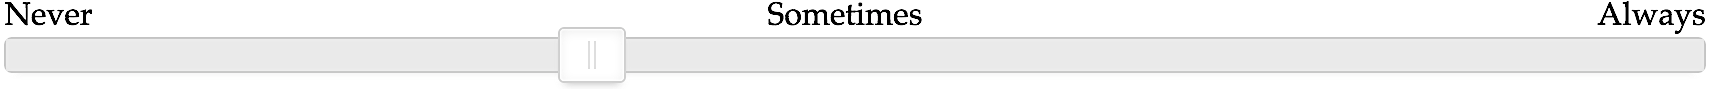
\includegraphics[width=\textwidth]{slider.png}
\caption{\label{fig:slider} This is a slider, as used by experiment participants.}
\end{figure}

Prior to seeing any experimental items, participants were given several practice questions, unrelated to the experimental stimuli, which also used continuous sliding scales ranging from \textit{Never} to \textit{Always} (or similar). Unlike the experimental stimuli, these questions had `correct' answers -- such as \textit{How likely is a fair coin to come up heads twice, if flipped 10 times? (very unlikely--very likely)}. If participants provided responses that could not be judged reasonably accurate, they were asked to re-read the instructions, and respond again, before they were able to proceed. This ensured that they were able to follow instructions, and were less likely to guess randomly throughout the experiment. There were no `accurate' answers in the experiment itself. All points on the response scale were associated with a number ranging from 0 (\textit{Never}) to 100 (\textit{Always}). 

\textbf{\textit{Pre-utterance beliefs}}, or baseline beliefs regarding activity habituality, were estimated from responses to stimuli presented without the activity description (see the next section for a more detailed explanation). The responses, aside from setting baseline measures (\textit{pre-utterance beliefs}) of activity habituality, also provide an additional norming measure for how likely it is that a particular activity would be engaged in, in the context of a given script. Thus, activities which are more or less habitual, within a given class, can be compared against one another.

\textbf{\textit{Post-utterance beliefs}} regarding activity habituality were estimated from responses to stimuli which included the redundant or non-redundant utterance (activity description), or where the activity description/utterance was visible.

\textbf{\textit{Belief change}} due to reading the activity description was determined by modeling the magnitude and direction of difference between \textit{pre-utterance beliefs} and \textit{post-utterance beliefs}.

\subsubsection{Procedure}

Participants were asked to read 6 experimental stimuli randomly selected out of the total of 24, as well as 4 filler items\footnote{To note, this means that each participant saw each manipulation only once, and the number of fillers was equal to the number of stimuli presented with dialogue.}.  Each condition was only presented once, as follows. 2 of the stories were presented without the dialogue and event description (context and setting up of common ground only), and 4 stories were presented in their entirety (context, setting up of common ground, and the dialogue/event description). The 2 partial stories allowed us to collect measures of \textit{pre-utterance beliefs} regarding activity habituality, and the 4 full stories gave us measures of \textit{post-utterance beliefs} conditioned on the event description. 

\begin{longtable}{|p{0.48\linewidth}|p{0.48\linewidth}|}
\hline
\textsc{Subject 1}: \textit{pre-utterance} belief & \textsc{Subject 2} \textit{post-utterance} belief\\
\hline
\hline
$<$context$>$ & $<$context$>$\\
&\\
$<$setting up of common ground$>$ & $<$setting up of common ground$>$\\
&\\
& $<$dialogue$>$\\
\hline
\textbf{\#. $<$habituality question$>$} & \textbf{\#. $<$habituality question$>$}\\
\hline
\end{longtable}

\normalsize
\addtocounter{table}{-1}

The experiment thus employed a between-subject design for belief measures, where \textit{pre-utterance} and \textit{post-utterance} belief estimates for any given item were provided by different participants, to eliminate the possibility of participants conditioning their \textit{post-utterance} estimates not only on inferences made from the text, but also on their own \textit{pre-utterance} estimates\footnote{However, the results below largely mirror the results of a within-subjects version of the study reported in \citet{Kravtchenko2015}.}. The 4 filler stimuli had the same structure as above, but with the dialogue portion replaced by script-neutral utterances: ``\textit{You know, I'm really tired.}", ``\textit{Hey, do you know what time it is?}", ``\textit{So, what are you up to?}", or ``\textit{Have you heard the news today yet?}".

\subsection{Results}

For the purposes of determining whether participants made any inferences regarding activity habituality, we modeled \textit{belief change}, i.e. the difference between \textit{pre-utterance} and \textit{post-utterance} beliefs, or activity habituality estimates made with and without seeing the activity description. \textit{Conventionally habitual} and \textit{non-habitual} activities were modeled separately, as the conventionally \textit{non-habitual} activity was used primarily as a control, and manipulations of common ground context did not otherwise target it. All factors were effect/sum coded. 

\subsubsection{\textit{Conventionally habitual} activities$\quad$('Paid the cashier')}

\textit{Pre-utterance belief} ratings (obtained from participants who did not see the activity descriptions) showed that \textit{ordinary} context activities are perceived as highly habitual (%
85.79
 on a 0-100 scale). As predicted, \textit{post-utterance belief} ratings (obtained from participants who saw the here, redundant, event descriptions) show lower habituality for the \textit{ordinary context} activities (%
72.37
) than \textit{pre-utterance belief} ratings.

\textit{Wonky} context activities (i.e., the condition where the \textit{conventionally habitual} activity was made non-habitual by the common ground context) are perceived as relatively non-habitual a priori (%
48
), and there was little change in participants' ratings (%
45.71
 for \textit{post-utterance beliefs}).  The results are illustrated in Fig. \ref{fig:exp1habitual}, using violin plots.

A linear mixed effects regression analysis, the results of which are summarized in Table \ref{tab:exp1habitual}, showed that the interaction between context and belief measure is statistically reliable ($\beta$=%
-10.77
, $p$<%
.001
). This interaction is driven by lowered activity habituality ratings when the readers see the utterance in a \textit{ordinary} context ($\beta$=%
-13.21
, $p$<%
.001
).

In this experiment as well as the two following experiments, we used linear mixed effects models with the maximal random effects structure that was justified by the design. This means that we included by-subject random intercepts and slopes for common ground context (\textit{ordinary} / \textit{wonky}) and belief measure (\textit{pre-utterance} / \textit{post-utterance}), as well as by-item random intercepts and slopes for both factors and their interaction \citep{Barr2013}. By-subject random slopes for the interaction were not included in the model, because we did not have any repeated measures for the interaction (each subject saw each condition only once). \textit{P}-values were obtained using the Satterthwaite approximation for degrees of freedom, as implemented in the lmerTest package \citep{Kuznetsova2017}.

%latex.default(coefs, file = "", title = "", table.env = TRUE,     booktabs = TRUE, caption = "Experiment 1: \\textit{conventionally habitual} (\\textit{cashier-paying}) activity analysis. This table shows the beta coefficients associated with each main effect in the model, as well as corresponding standard errors, \\emph{t}-values, and significance levels.",     label = "tab:exp1habitual", where = "ht")%
\begin{table}[ht]
\caption{Experiment 1: \textit{conventionally habitual} (\textit{cashier-paying}) activity analysis. This table shows the beta coefficients associated with each main effect in the model, as well as corresponding standard errors, \emph{t}-values, and significance levels.\label{tab:exp1habitual}} 
\begin{center}
\begin{tabular}{lrrrl}
\toprule
\multicolumn{1}{l}{}&\multicolumn{1}{c}{$\beta$}&\multicolumn{1}{c}{SE($\beta$)}&\multicolumn{1}{c}{\textbf{t}}&\multicolumn{1}{c}{\textbf{p}}\tabularnewline
\midrule
Intercept&$ 63.03$&$1.84$&$34.32$&\textbf{\textless .001}\tabularnewline
Common Ground: Ordinary&$ 32.38$&$3.33$&$ 9.72$&\textbf{\textless .001}\tabularnewline
Belief: Post-utterance&$ -7.83$&$1.71$&$-4.58$&\textbf{\textless .001}\tabularnewline
Common Ground * Belief&$-10.77$&$2.40$&$-4.50$&\textbf{\textless .001}\tabularnewline
\bottomrule
\end{tabular}\end{center}
\end{table}


\begin{knitrout}
\definecolor{shadecolor}{rgb}{0.969, 0.969, 0.969}\color{fgcolor}\begin{figure}
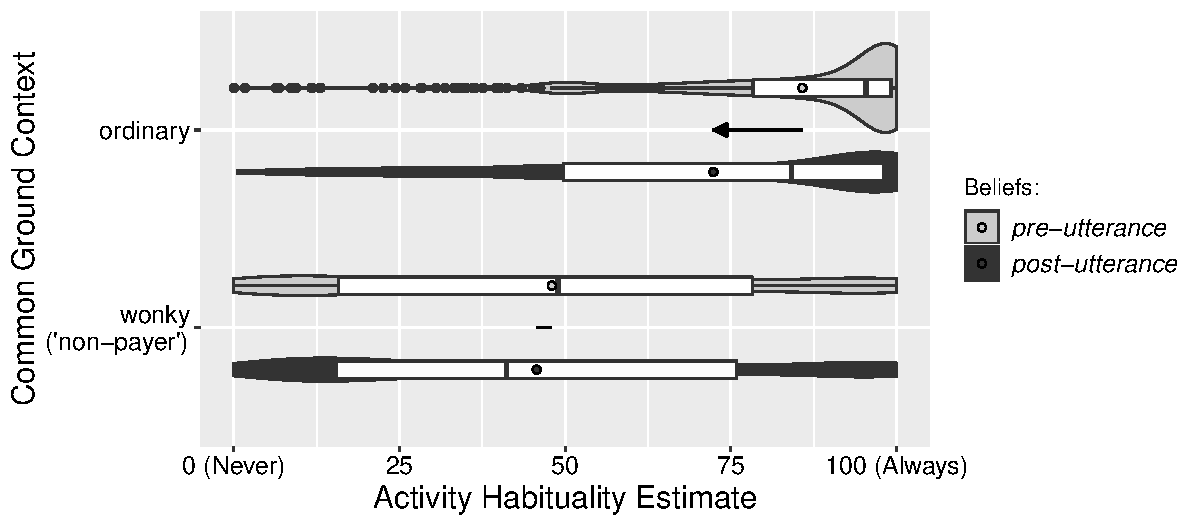
\includegraphics[width=\maxwidth]{figure/unnamed-chunk-15-1} \caption{\label{fig:exp1habitual}Experiment 1: \textit{conventionally habitual} (\textit{cashier-paying}) activity analysis. This plot shows changes in activity habituality estimates depending on whether the utterance is seen, as well as whether the context causes the utterance activity to be perceived as non-habitual. Violin plots, overlaid with box plots, show the distribution of estimates.  A violin plot is simply a smoothed and mirrored histogram: the fatter the distribution at a given point, the more instances there are of that particular activity habituality estimate.  Circles represent mean values. Arrows show statistically significant differences between \textit{before/pre-utterance} and \textit{after/post-utterance} ratings.}\label{fig:unnamed-chunk-15}
\end{figure}


\end{knitrout}

These results show that, as predicted, when a \textit{conventionally habitual} activity is explicitly described in a \textit{ordinary} common ground context (i.e. a context in which the activity can be automatically inferred), many readers infer that the \textit{conventionally habitual} activity must in fact be \textit{non-habitual}; i.e., unusual for the individual who is the subject of the story, and therefore worth mentioning explicitly.

\subsubsection{Conventionally \textit{non-habitual} activities$\quad$('Bought some apples')}

There was little change in participants' ratings of conventionally \textit{non-habitual} activities from \textit{pre-utterance beliefs} to \textit{post-utterance beliefs} (\textit{ordinary}: %
40.8
 to %
42.47
; \textit{wonky}: %
38.49
 to %
39.56
), see Fig. \ref{fig:exp1nonhabitual}.

A linear mixed effects regression analysis showed that estimates of activity habituality do not vary with the common ground context, nor are they conditioned on the utterance describing the activity (see Table \ref{tab:exp1nonhabitual}). This is also consistent with our predictions, and indicates both that the context alteration does not inherently cause a change in activity habituality estimates (regardless of how script-central the activity is), and that conventionally \textit{non-habitual} activities, given our \textit{ordinary} context, are not interpreted as less habitual when mentioned.

%latex.default(coefs, file = "", title = "", table.env = TRUE,     booktabs = TRUE, caption = "Experiment 1: conventionally \\textit{non-habitual} (\\textit{apple-buying}) activity analysis.",     label = "tab:exp1nonhabitual", where = "ht")%
\begin{table}[ht]
\caption{Experiment 1: conventionally \textit{non-habitual} (\textit{apple-buying}) activity analysis.\label{tab:exp1nonhabitual}} 
\begin{center}
\begin{tabular}{lrrrl}
\toprule
\multicolumn{1}{l}{}&\multicolumn{1}{c}{$\beta$}&\multicolumn{1}{c}{SE($\beta$)}&\multicolumn{1}{c}{\textbf{t}}&\multicolumn{1}{c}{\textbf{p}}\tabularnewline
\midrule
Intercept&$40.29$&$1.86$&$21.69$&\textbf{\textless .001}\tabularnewline
Common Ground: Ordinary&$ 2.88$&$2.07$&$ 1.39$&0.2\tabularnewline
Belief: Post-utterance&$ 1.34$&$1.85$&$ 0.73$&0.5\tabularnewline
Common Ground * Belief&$ 0.01$&$2.14$&$ 0.01$&1\tabularnewline
\bottomrule
\end{tabular}\end{center}
\end{table}


\begin{knitrout}
\definecolor{shadecolor}{rgb}{0.969, 0.969, 0.969}\color{fgcolor}\begin{figure}
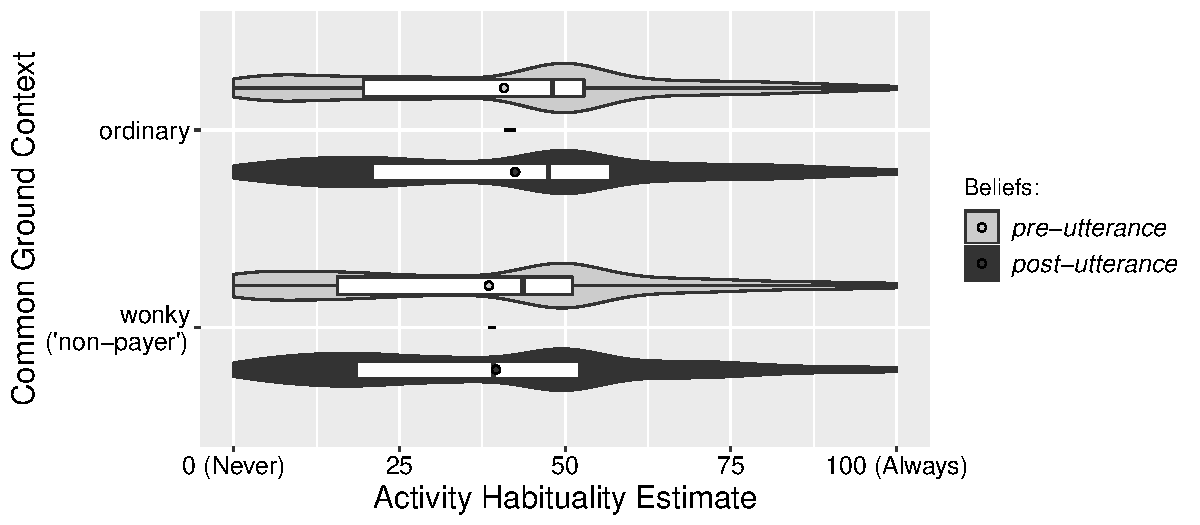
\includegraphics[width=\maxwidth]{figure/unnamed-chunk-20-1} \caption{\label{fig:exp1nonhabitual}Experiment 1: conventionally \textit{non-habitual} (\textit{apple-buying}) activity analysis.}\label{fig:unnamed-chunk-20}
\end{figure}


\end{knitrout}

\subsection{Discussion}

The results of the first experiment indicate that comprehenders do in fact perceive informational redundancy, in the form of mention of overly habitual activities, as a possible violation of conversational norms, and that they resolve this violation by reinterpreting the activities described as non-habitual. On average, participants rate conceptually predictable activities as less habitual if they see them mentioned overtly, in contrast to all other activities. In other words, comprehenders react to redundancy as they typically do to other apparent maxim violations -- by assuming an implied non-literal meaning, or alternate background world state, that resolves the apparent violation. This runs in some contradiction to the initial ambivalence \citet{Grice1975} expressed about the existence of such a constraint, and equivocal evidence from studies of informationally redundant nominal modification. 

These results rule out the ``no inference" hypothesis outlined in Section \ref{how-might-comprehenders-react-to-informational-redundancy}, and raise two questions that we address in the following experiments, regarding the importance of (implicit) prosody, and that the speaker signaling intentionality of the activity description. First, an exclamation point may serve multiple purposes: it may signal surprise as to the course of described events, a speaker's intentionality in communicating a piece of information\footnote{I.e., the speaker displays clear and conscious intent to draw to the comprehender's attention the face that a given event occurred – as opposed to stalling for time, thinking of something to say, aborting a previously planned utterance, simply being uncooperative, and so forth.}, the importance and relevance of the information conveyed to the general discourse and comprehender's interests, and that the information preceding the exclamation point constitutes an ``encapsulated" message in its own right (rather than serving as a temporal or causal anchor\footnote{For example: \textit{He paid the cashier. Then he noticed it was his classmate.}}). Although it could be argued that the exclamation point \citep[often a signal of surprise;][]{Rett2011} forces a relative `non-habitual activity' interpretation independent of utterance informativity, this is not a likely explanation, as no signs of a similar effect are present in any of the other conditions. 

Therefore, the first question is: how generalizable is the effect, and does the inference arise in contexts that do not implicitly signal the unexpectedness of the information conveyed (beyond the point that it is mentioned at all)? There is relatively little work on the question of which contextual cues specifically people employ in computing context-dependent inferences, as well as how these cues influence final interpretation. To test this, in Experiment 2 we use a discourse marker ("\textit{Oh yeah, and...}") which does not clearly signal surprise -- but does frame the event description as intentionally conveyed, as important/relevant to the topic at hand, and as an ``encapsulated message." 

The second question raised is whether informational redundancy itself is sufficient to trigger such an inference. As mentioned previously, we start from the premise that rational speakers mention only that which cannot be automatically inferred by the comprehender. A charitable comprehender may be expected to expend considerable effort on rescuing the assumption of a cooperative or rational speaker \citep{Davidson1974}. If only activities under a certain threshold of habituality deserve mention, then comprehenders should conclude that the activity mentioned is relatively unusual, independently of any special emphasis on the utterance.  In general, most types of inferences, if they occur, should occur as long as the semantic content of the utterance remain constant (cf. the ``non-detachability" hypothesis).

On the other hand, pragmatic inferences must be calculable \citep{Levinson2000}, and utterances must be attended to closely enough in the first place, before they may trigger any inferences \citep{Wilson2004}. That is, particularly for non-generalized (context-sensitive) inferences, the context must offer sufficient support that the reader can infer the speaker's intent, or a plausible background state, with reasonable certainty.  It's not clear, in our case, if the blatant redundancy itself constitutes sufficient support. Likewise, while rational speakers may only mention activities that are not easily inferable, forcing a comprehender to expend significant effort on recovering an utterance's intended meaning or significance is not particularly rational behavior. The degree of ``intentionality" on the part of the speaker (also signaled in our stimuli by the exclamation mark) may affect comprehenders' willingness and effort in guessing any implied meaning, as an utterance that may be a stray thought uttered without any specific intent may not be worth much effort to attempt to decipher (cf. the ``form sensitivity" hypothesis). To test whether informational redundancy itself is sufficient for triggering the inference, or whether some amount of discourse or prosodic emphasis is necessary for its generation, in Experiment 3 we present readers with the same task and stimuli, but strip the event description of prosodic or discourse cues signaling speaker intentionality.

\section{Experiment 2: Implicit Discourse Support}\label{exp2}



The second experiment tests whether the effect, of informationally redundant event descriptions being interpreted by readers as signaling activity \textit{non-habituality}, is generalizable. To do so, we can replace the exclamation point with a non-prosodic discourse marker that signals speaker intentionality and utterance relevance (but crucially, not surprise). In this experiment, we frame the informationally redundant event description as an apparent recalling of information specifically intended to be mentioned to the comprehender, and implicitly relevant to the material just discussed: ``\textit{Oh yeah, and [he paid the cashier]}."

This discourse marker does not clearly signal surprise at the activity having been engaged in, nor does it explicitly support the intended inference otherwise -- and in contrast to the exclamation mark in Exp.1, is a non-prosodic manipulation of the event description. We therefore consider it a good test of whether the effect generalizes beyond the specific context used in the first experiment.

\subsection{Methods}

\subsubsection{Participants}

700 eligible participants (%
787
 total; median age bracket %
26-35
; %
51.3
\% female) were recruited on Amazon Mechanical Turk. %
87
 participants were excluded from analysis (%
11.05
\%), following the same exclusion criteria as applied in Experiment 1.

\subsubsection{Design}

The design of this experiment was motivated by the same considerations as Experiment 1 -- with the exception of how the event description was framed. Instead of marking the target utterance with an exclamation mark, we framed the same utterance as a piece of information the speaker had just recalled, apparently having previously intended to mention it to the comprehender:

\ex. ``John just came back from the grocery store.  \textbf{Oh yeah, and he paid the cashier.}"

The \textit{oh yeah...} discourse marker does not conventionally signal surprise, and therefore does not potentially signal the specific inference that we are testing for. It does, however, imply speaker intent behind conveying precisely this message, the importance and relevance of the message to the current discourse and comprehender -- as well as that the message stands alone, and is not intended to simply serve as causal or temporal scaffolding for a further message/event.

\subsubsection{Materials}

The same 24 stimuli were used as in Exp. 1. In this case, the critical utterance was prepended by ``\textit{Oh yeah, and...}":

\ex.\label{ex:habitual2} \centering\textsc{Ordinary context}
\vspace{-0.1cm}
\centering

\begin{longtable}{p{0.435\textwidth}|p{0.435\textwidth}}
\multicolumn{2}{p{0.9\textwidth}}{$[$1$]$ John often goes to the grocery store around the corner from his apartment.} \\
\hline
\multicolumn{2}{p{0.9\textwidth}}{$[$2$]$ Recently, he came home from the store with groceries.  When he came in, he saw his roommate Susan in the hallway, and started talking to her about his trip to the store.  As he went to the kitchen to put his groceries away, Susan went to the living room, where their roommate Peter was watching TV.} \\
\hline
\multicolumn{2}{p{0.9\textwidth}}{$[$3$]$ Susan said to Peter: ``John just came back from the grocery store.} \\
\hline
$[$4a$]$ \textbf{Oh yeah, and} he \textit{paid the \mbox{cashier\textsubscript{habitual}}}.'' & $[$4b$]$ \textbf{Oh yeah, and} he \textit{got some apples\textsubscript{non-habitual}}.''
\end{longtable}
\addtocounter{table}{-1}

\subsubsection{Procedure}

The procedure was identical to that of Exp. 1.

\subsubsection{Measures}

The same response measures as in Exp. 1 were used to estimate \textit{pre-utterance beliefs} and \textit{post-utterance beliefs}. 

\subsection{Results}


As in Experiment 1, to determine whether participants made inferences regarding activity habituality, we modeled \textit{belief change} - the difference between \textit{pre-utterance} and \textit{post-utterance} beliefs. \textit{Conventionally habitual} and conventionally \textit{non-habitual} activities were again modeled separately. All factors were effect/sum coded. 

\subsubsection{\textit{Conventionally habitual} activities}

As we predicted, \textit{pre-utterance belief} ratings for \textit{ordinary context} activities showed that these activities are judged to be highly habitual (%
84.71
). As in Experiment 1, \textit{post-utterance beliefs} about the habituality of \textit{ordinary context} activities were significantly lower (%
73.84
), and \textit{wonky} common ground estimates remained stable (%
47.45
 \textit{pre-utterance} to %
47.47
 \textit{post-utterance}).

A linear mixed effects regression analysis, the results of which are summarized in Table \ref{tab:exp2habitual}, showed an interaction between context and belief measure ($\beta$=%
-11.71
, $p$<%
.001
), which is driven by lowered activity habituality ratings when the readers see the utterance in a ordinary context ($\beta$=%
-11.11
, $p$<%
.001
). All model specifications are as described in Exp. 1.  A plot illustrating the interaction can be seen in Fig. \ref{fig:exp2habitual}, which shows a pattern of results that is remarkably quantitatively and qualitatively similar to that of Exp. 1.  Exp. 1 and 2 are compared directly, and to Exp. 3, in Section \ref{cross-experiment-analysis-and-gradience-of-the-non-habituality-effect}.

%latex.default(coefs, file = "", title = "", table.env = TRUE,     booktabs = TRUE, caption = "Experiment 2: \\textit{conventionally habitual} (\\textit{cashier-paying}) activity analysis.",     label = "tab:exp2habitual", where = "ht")%
\begin{table}[ht]
\caption{Experiment 2: \textit{conventionally habitual} (\textit{cashier-paying}) activity analysis.\label{tab:exp2habitual}} 
\begin{center}
\begin{tabular}{lrrrl}
\toprule
\multicolumn{1}{l}{}&\multicolumn{1}{c}{$\beta$}&\multicolumn{1}{c}{SE($\beta$)}&\multicolumn{1}{c}{\textbf{t}}&\multicolumn{1}{c}{\textbf{p}}\tabularnewline
\midrule
Intercept&$ 63.58$&$1.85$&$34.33$&\textbf{\textless .001}\tabularnewline
Common Ground: Ordinary&$ 31.60$&$3.35$&$ 9.43$&\textbf{\textless .001}\tabularnewline
Belief: Post-utterance&$ -5.31$&$1.38$&$-3.83$&\textbf{\textless .001}\tabularnewline
Common Ground * Belief&$-11.71$&$2.03$&$-5.76$&\textbf{\textless .001}\tabularnewline
\bottomrule
\end{tabular}\end{center}
\end{table}


\begin{knitrout}
\definecolor{shadecolor}{rgb}{0.969, 0.969, 0.969}\color{fgcolor}\begin{figure}
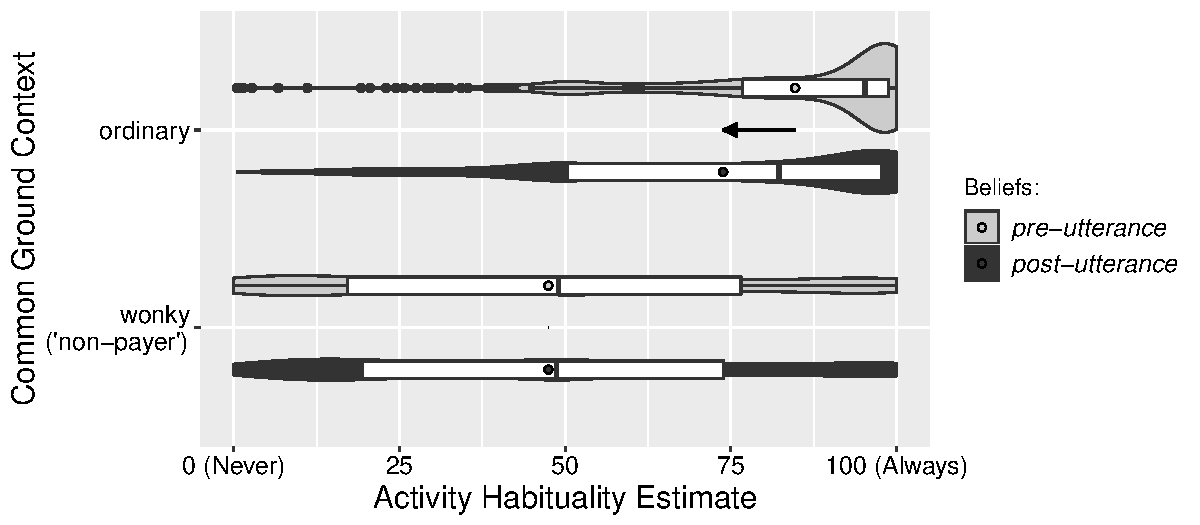
\includegraphics[width=\maxwidth]{figure/unnamed-chunk-34-1} \caption{\label{fig:exp2habitual}Experiment 2: \textit{conventionally habitual} (\textit{cashier-paying}) activity analysis.}\label{fig:unnamed-chunk-34}
\end{figure}


\end{knitrout}

These results support our prediction that readers perceive informationally redundant utterances as abnormal, and make pragmatic inferences (of activity \textit{non-habituality}), regardless of whether implicit prosody or other markers conventionally associated with surprisal are present.

\subsubsection{Conventionally \textit{non-habitual} activities}

In contrast to Experiment 1, there was some increase in participants' ratings of conventionally \textit{non-habitual} activities from \textit{pre-utterance beliefs} (\textit{ordinary}: %
40.3
 to %
43.22
; \textit{wonky}: %
37.74
 to %
43.05
), see Fig. \ref{fig:exp2nonhabitual}.

A linear mixed effects regression analysis showed that estimates of activity habituality increase slightly when the utterance describing the conventionally \textit{non-habitual} activity (see Table \ref{tab:exp2nonhabitual}) is visible ($\beta$=%
5.09
, $p$<%
.01
).

While not identical to the results of the first experiment (which showed a slight numerical increase in rating only), this is consistent with a peripheral prediction we made prior to running the experiments: simply mentioning a non-habitual, or non-redundant activity may increase the perception of its habituality, by providing some evidence that, e.g., \textit{John} is at least an occasional \textit{apple purchaser}. As the direction of this effect does not change our interpretation of the results, we leave it aside for future exploration.

%latex.default(coefs, file = "", title = "", table.env = TRUE,     booktabs = TRUE, caption = "Experiment 2: conventionally \\textit{non-habitual} (\\textit{apple-buying}) activity analysis.",     label = "tab:exp2nonhabitual", where = "ht")%
\begin{table}[ht]
\caption{Experiment 2: conventionally \textit{non-habitual} (\textit{apple-buying}) activity analysis.\label{tab:exp2nonhabitual}} 
\begin{center}
\begin{tabular}{lrrrl}
\toprule
\multicolumn{1}{l}{}&\multicolumn{1}{c}{$\beta$}&\multicolumn{1}{c}{SE($\beta$)}&\multicolumn{1}{c}{\textbf{t}}&\multicolumn{1}{c}{\textbf{p}}\tabularnewline
\midrule
Intercept&$40.99$&$1.85$&$22.14$&\textbf{\textless .001}\tabularnewline
Common Ground: Ordinary&$ 0.95$&$1.83$&$ 0.52$&0.6\tabularnewline
Belief: Post-utterance&$ 5.09$&$1.78$&$ 2.86$&\textbf{\textless .01}\tabularnewline
Common Ground * Belief&$-1.22$&$1.55$&$-0.79$&0.4\tabularnewline
\bottomrule
\end{tabular}\end{center}
\end{table}


\begin{knitrout}
\definecolor{shadecolor}{rgb}{0.969, 0.969, 0.969}\color{fgcolor}\begin{figure}
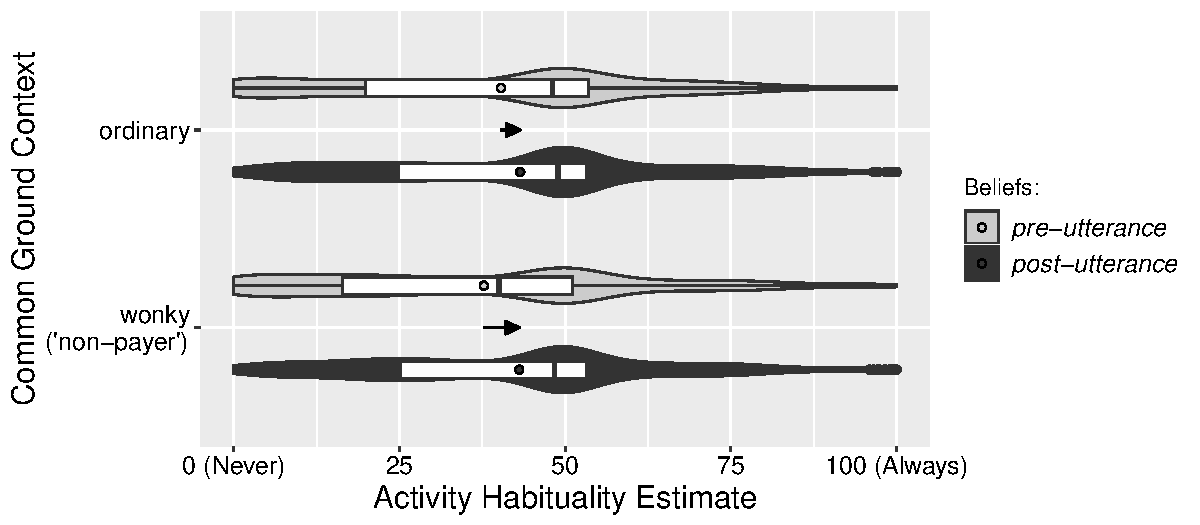
\includegraphics[width=\maxwidth]{figure/unnamed-chunk-41-1} \caption{\label{fig:exp2nonhabitual}Experiment 2: conventionally \textit{non-habitual} (\textit{apple-buying}) activity analysis.}\label{fig:unnamed-chunk-41}
\end{figure}


\end{knitrout}

\subsection{Discussion}

Together with Experiment 1, these results show that readers find informational redundancy abnormal at face value, and make pragmatic inferences to reconcile apparent informational redundancy with their expectations of utterance utility. This further disconfirms the "no inference" hypothesis, and indicates that the effect is generalizable, and not dependent on conventional indicators of activity non-habituality, such as implicit exclamatory intonation.

The results of Experiments 1 and 2, however, do not permit us to distinguish between the 2nd and 3rd hypotheses ("non-detachability" vs. "form sensitivity"), as they leave open the question of whether the \textit{non-habituality} effect is dependent on some degree of intentionality-signaling, or applies independently of discourse context. Experiment 2 provides some support for the "non-detachability" hypothesis, as the magnitude of the inference remains entirely stable, even as the form of intention or relevance signaling is substantially changed.

If the effect is dependent on some amount of relevance or intentionality signaling, this would support the "form sensitivity" hypothesis over the "non-detachability" hypothesis, by suggesting one of the following. Comprehenders may be relatively unwilling to expend substantial effort on decoding a plausible inference in the absence of evidence that doing so is worth it, and that the utterance has some amount of import. Similarly, they may stop short in their efforts, on the assumption that it is more likely that speakers would occasionally violate this particular conversational maxim, than that they would provide insufficient evidence that the utterance communicates something of note. Finally, they may simply be generally tolerant of informational redundancy, unless context suggests that the redundancy has a `point.' Experiment 3 presents the same task and materials to participants, but removes the prosody or discourse markers that signal relevance and speaker intent.

\section{Experiment 3: Removing Contextual Support}\label{exp3}



To investigate whether explicitly signaling speaker intent has an influence on the strength of the \textit{non-habituality} effect, we designed a third experiment which differs only in the absence of special prosodic or discourse markers, or evidence for the relevance/informativity of the activity description. Our prediction is that while the effect may be attenuated somewhat, comprehenders should nevertheless make a measurable attempt to compensate for a violation in expected informational utility (i.e., while there may be some degree of "form sensitivity," the inference should nevertheless arise).

\subsection{Methods}

\subsubsection{Participants}

700 eligible participants (%
759
 total; median age bracket %
26-35
; %
51.6
\% female) were recruited on Amazon Mechanical Turk. %
59
 participants were excluded from analysis (%
7.77
\%), following the same exclusion criteria as applied as in previous experiments.

\subsubsection{Design}

The design was motivated by the same factors as Experiments 1 and 2, but all markers of relevance were removed from the activity description: 

\ex. "John just came back from the grocery store.  \textbf{He paid the cashier.}"

In this case, there is no clear signal indicating the relevance or informativity of the utterance. One could plausibly imagine the event description, in this case, to be `filler material,' only semi-intentionally uttered while the speaker is planning what to say next, or as (planned, but then possibly abandoned) temporal or causal scaffolding for a more important event to be described, such as in:

\ex.\label{anchor} "John just came back from the grocery store.  He paid the cashier.  \textit{He then realized he'd forgotten his driver's license!}"

\subsubsection{Materials}

The same 24 stimuli were used as in the previous experiments. The only alteration from Experiment 1 was the substitution of the exclamation point with a period: 

\ex.\label{ex:habitual3} \centering\textsc{Ordinary context}
\vspace{-0.1cm}
\centering

\begin{longtable}{p{0.435\textwidth}|p{0.435\textwidth}}
\multicolumn{2}{p{0.9\textwidth}}{$[$1$]$ John often goes to the grocery store around the corner from his apartment.} \\
\hline
\multicolumn{2}{p{0.9\textwidth}}{$[$2$]$ Recently, he came home from the store with groceries.  When he came in, he saw his roommate Susan in the hallway, and started talking to her about his trip to the store.  As he went to the kitchen to put his groceries away, Susan went to the living room, where their roommate Peter was watching TV.} \\
\hline
\multicolumn{2}{p{0.9\textwidth}}{$[$3$]$ Susan said to Peter: ``John just came back from the grocery store.} \\
\hline
$[$4a$]$ He \textit{paid the \mbox{cashier\textsubscript{habitual}}}.'' & $[$4b$]$ He \textit{got some apples\textsubscript{non-habitual}}.''
\end{longtable}
\addtocounter{table}{-1}

\subsubsection{Procedure}

The procedure was identical to that of previous experiments. 

\subsubsection{Measures}

The same response measures as in the previous experiments were used to estimate \textit{pre-utterance beliefs} and \textit{post-utterance beliefs}. 

\subsection{Results}

As in previous experiments, we modeled the difference between \textit{pre-utterance} and \textit{post-utterance} beliefs. \textit{Conventionally habitual} and conventionally \textit{non-habitual} activities were modeled separately. All factors were effect/sum coded. 

\subsubsection{\textit{Conventionally habitual} activities}

As in the previous experiments, \textit{pre-utterance belief} ratings showed \textit{ordinary context} activities to be highly habitual (%
85.59
), and \textit{wonky context} activities to be less habitual (%
49.5
). Consistent with our predictions, \textit{post-utterance beliefs} are significantly lower in the \textit{ordinary context condition} (%
80.3
), but less so than in the previous two experiments. Exp. 3 is compared directly to Exp. 1 and 2 in Section \ref{cross-experiment-analysis-and-gradience-of-the-non-habituality-effect}.

A linear mixed effects regression analysis, the results of which are summarized in Table \ref{tab:exp3habitual}, showed an interaction between context and belief measure ($\beta$=%
-5.4
, $p$<%
.01
), which is driven by lowered activity habituality ratings when the readers see the utterance in an ordinary context ($\beta$=%
-4.87
, $p$<%
.001
). All model specifications are as described in Exp. 1 and 2.  A plot illustrating the interaction can be seen in Fig. \ref{fig:exp3habitual}.

%latex.default(coefs, file = "", title = "", table.env = TRUE,     booktabs = TRUE, caption = "Experiment 3: \\textit{conventionally habitual} (\\textit{cashier-paying}) activity analysis.",     label = "tab:exp3habitual", where = "ht")%
\begin{table}[ht]
\caption{Experiment 3: \textit{conventionally habitual} (\textit{cashier-paying}) activity analysis.\label{tab:exp3habitual}} 
\begin{center}
\begin{tabular}{lrrrl}
\toprule
\multicolumn{1}{l}{}&\multicolumn{1}{c}{$\beta$}&\multicolumn{1}{c}{SE($\beta$)}&\multicolumn{1}{c}{\textbf{t}}&\multicolumn{1}{c}{\textbf{p}}\tabularnewline
\midrule
Intercept&$66.38$&$1.88$&$35.40$&\textbf{\textless .001}\tabularnewline
Common Ground: Ordinary&$33.21$&$3.40$&$ 9.77$&\textbf{\textless .001}\tabularnewline
Belief: Post-utterance&$-2.20$&$0.93$&$-2.36$&\textbf{\textless .05}\tabularnewline
Common Ground * Belief&$-5.40$&$1.75$&$-3.10$&\textbf{\textless .01}\tabularnewline
\bottomrule
\end{tabular}\end{center}
\end{table}


\begin{knitrout}
\definecolor{shadecolor}{rgb}{0.969, 0.969, 0.969}\color{fgcolor}\begin{figure}
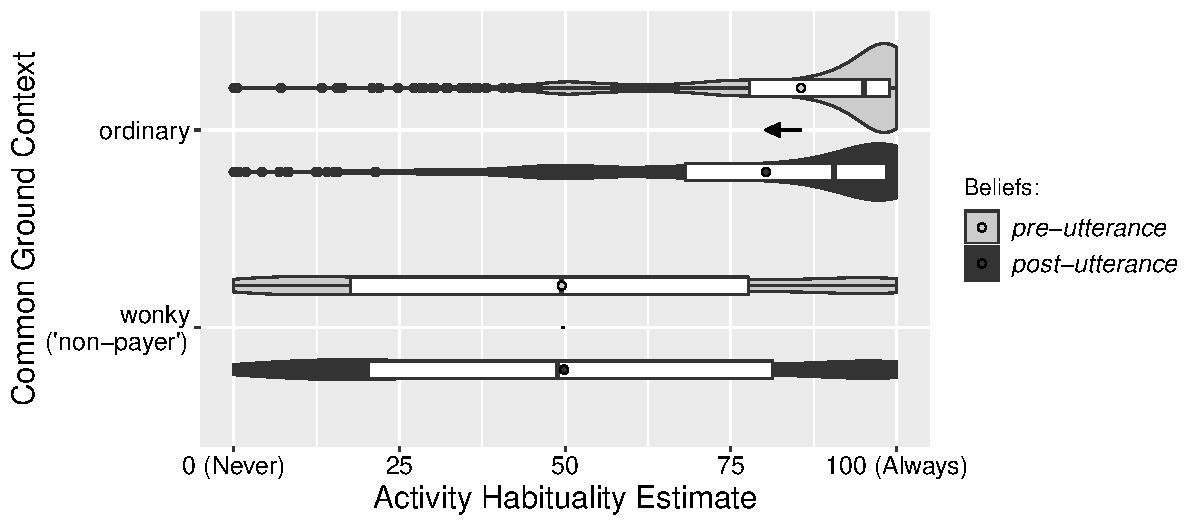
\includegraphics[width=\maxwidth]{figure/unnamed-chunk-54-1} \caption{\label{fig:exp3habitual}Experiment 3: \textit{conventionally habitual} (\textit{cashier-paying}) activity analysis.}\label{fig:unnamed-chunk-54}
\end{figure}


\end{knitrout}

These results indicate that, consistent with our predictions and the results of Exp. 1 and 2, when an easily inferable activity is overtly mentioned in a \textit{ordinary} common ground context, comprehenders do infer some degree of activity non-habituality, even without implicit prosody or discourse markers putting additional emphasis on the utterance.

\subsubsection{Conventionally \textit{non-habitual} activities}

In contrast to Experiment 1 and similar to Experiment 2, there was some increase in participants' ratings of conventionally \textit{non-habitual} activities from \textit{pre-utterance} to \textit{post-utterance} beliefs (\textit{ordinary}: %
41.08
 to %
46.46
; \textit{wonky}: %
37.61
 to %
44.42
), see Fig. \ref{fig:exp3nonhabitual}.

A linear mixed effects regression analysis showed that estimates of activity habituality do not vary with changes in the common ground context (or common ground \textit{wonkiness}), but do increase slightly when the utterance describing the conventionally \textit{non-habitual} activity (see Table \ref{tab:exp3nonhabitual}) is visible ($\beta$=%
6.88
, $p$<%
.001
).  As in the case of Exp. 2, we suspect that explicitly mentioning a relatively unusual activity leads participants to believe that activity to be slightly more habitual than they would otherwise assume.

%latex.default(coefs, file = "", title = "", table.env = TRUE,     booktabs = TRUE, caption = "Experiment 3: conventionally \\textit{non-habitual} (\\textit{apple-buying}) activity analysis.",     label = "tab:exp3nonhabitual", where = "ht")%
\begin{table}[ht]
\caption{Experiment 3: conventionally \textit{non-habitual} (\textit{apple-buying}) activity analysis.\label{tab:exp3nonhabitual}} 
\begin{center}
\begin{tabular}{lrrrl}
\toprule
\multicolumn{1}{l}{}&\multicolumn{1}{c}{$\beta$}&\multicolumn{1}{c}{SE($\beta$)}&\multicolumn{1}{c}{\textbf{t}}&\multicolumn{1}{c}{\textbf{p}}\tabularnewline
\midrule
Intercept&$42.12$&$2.12$&$19.84$&\textbf{\textless .001}\tabularnewline
Common Ground: Ordinary&$ 2.29$&$2.41$&$ 0.95$&0.4\tabularnewline
Belief: Post-utterance&$ 6.88$&$1.77$&$ 3.88$&\textbf{\textless .001}\tabularnewline
Common Ground * Belief&$-1.39$&$1.72$&$-0.81$&0.4\tabularnewline
\bottomrule
\end{tabular}\end{center}
\end{table}


\begin{knitrout}
\definecolor{shadecolor}{rgb}{0.969, 0.969, 0.969}\color{fgcolor}\begin{figure}
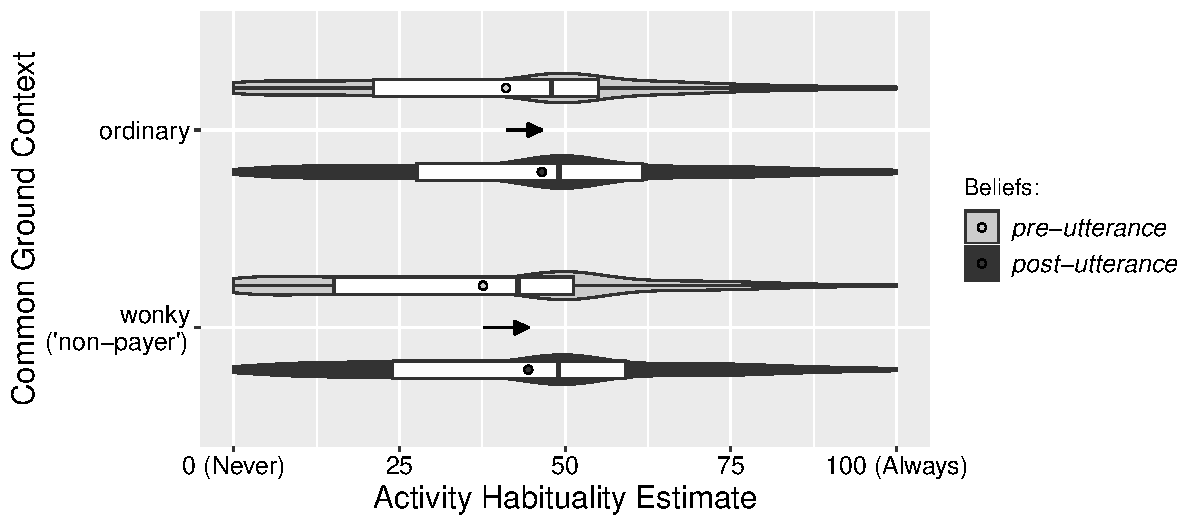
\includegraphics[width=\maxwidth]{figure/unnamed-chunk-61-1} \caption{\label{fig:exp3nonhabitual}Experiment 3: conventionally \textit{non-habitual} (\textit{apple-buying}) activity analysis.}\label{fig:unnamed-chunk-61}
\end{figure}


\end{knitrout}

\subsection{Discussion}

In contrast to the results of the first two experiments, these results suggest that, when informationally redundant utterances are presented without a signal of speaker intent and utterance relevance, comprehenders are relatively unlikely to draw \textit{non-habituality} inferences. This is consistent with the "form sensitivity" hypothesis described in Section \ref{how-might-comprehenders-react-to-informational-redundancy}, and the premise that, while rational speakers may typically avoid making utterances that have no literal or implied informational utility, and while such utterances may prompt pragmatic inferences on the part of comprehenders (which increase the informational utility of such utterances), such inferences are dependent on the degree to which the utterances are perceived as intentional.  Further, while the results are not consistent with a strong form of the "non-detachability" hypothesis, they do broadly suggest that redundancy generates inferences regardless of form of delivery.

We should note, however, that this is not what we found in the experiments we are replicating - where the inference disappeared entirely without prosodic or discourse emphasis (strongly supporting the "form sensitivity" hypothesis, and at odds with the "non-detachability" hypothesis).  Although the replicated experiments were not as highly powered, the difference might be due to stimulus redesign - in the supplementary materials\footnote{\url{https://osf.io/8fz4m/?view_only=ff5859d3f33b485d95254395f95a52dc}}, we speculate as to why this might be the case.

\section{Cross-Experiment Analysis and Gradience of the Habituality Effect}\label{cross-experiment-analysis-and-gradience-of-the-non-habituality-effect}



In this section, we directly compare the results of the three experiments.  We predict that informationally redundant utterances can trigger \textit{non-habituality} inferences of similar magnitude independently of whether one uses an explicit marker of suprisal: in other words, that the effect is generalizable.  However, we also predict that the effect is significantly attenuated in absence of a prosodic or discourse marker which signals relevance and speaker intent.

\subsection{\textit{Conventionally habitual} activities}

To directly compare the three experiments, we run a $3\times 2\times 2$ linear mixed effects regression analysis of \textit{conventionally habitual} activities.  We modeled \textit{belief change} (\textit{pre-utterance} vs. \textit{post-utterance} beliefs), as a function of common ground (\textit{ordinary} vs. \textit{wonky}), as well as the between-subject discourse marker manipulation ('\textit{!}' vs. `\textit{Oh yeah, and}' vs. `\textit{.}').  The first two factors were effect/sum coded.  We used Helmert coding for the 3-level experiment factor, as this allowed us to make the comparisons of theoretical interest: Exp. 1 vs. Exp. 2 ('\textit{!}' vs. `\textit{Oh yeah, and}'), and then Exp. 3 vs. Exp. 1 and 2 grouped together ('\textit{.}' vs. the relevance markers).

The regression analysis showed a significant three-way interaction between relevance marker presence, common ground context, and belief measure: there was a significantly smaller \textit{non-habituality} effect in Exp. 3 than in Experiments 1 and 2 ($\beta$=%
5.78
, $p$<%
.01
), and no significant difference between Experiments 1 and 2 ($\beta$=%
-0.6
, $p$=%
.80
).


We used the maximal converging model, with by-subject random intercepts and slopes for common ground context (\textit{ordinary} / \textit{wonky}) and belief measure (\textit{pre-utterance} / \textit{post-utterance}), by-item random intercepts and slopes for both factors and their interaction, and a by-item random slope for experiment. By-subject random slopes for the interaction were not included in the model due to lack of within-subject repeated measures. The random slope for the full (by-item) experiment by common ground by belief measure interaction was not included due to non-convergence. A plot illustrating the comparison can be seen in Fig. \ref{fig:expallhabitual}.

%latex.default(coefs, file = "", title = "", table.env = TRUE,     booktabs = TRUE, caption = "Experiments 1-3: \\textit{conventionally habitual} (\\textit{cashier-paying}) activity analysis.",     label = "tab:expall", where = "ht")%
\begin{table}[ht]
\caption{Experiments 1-3: \textit{conventionally habitual} (\textit{cashier-paying}) activity analysis.\label{tab:expall}} 
\begin{center}
\begin{tabular}{lrrrl}
\toprule
\multicolumn{1}{l}{}&\multicolumn{1}{c}{$\beta$}&\multicolumn{1}{c}{SE($\beta$)}&\multicolumn{1}{c}{\textbf{t}}&\multicolumn{1}{c}{\textbf{p}}\tabularnewline
\midrule
Intercept&$64.34$&$1.78$&$36.14$&\textbf{\textless .001}\tabularnewline
`!' vs. `Oh yeah...'&$ 0.49$&$0.86$&$ 0.57$&0.6\tabularnewline
`.' vs. Relevance Markers&$ 3.08$&$0.81$&$ 3.81$&\textbf{\textless .001}\tabularnewline
Common Ground: Ordinary&$32.40$&$3.22$&$10.05$&\textbf{\textless .001}\tabularnewline
Belief: Post-utterance&$-5.07$&$1.04$&$-4.86$&\textbf{\textless .001}\tabularnewline
`!' vs. `Oh yeah' * Common Ground&$-0.64$&$1.43$&$-0.45$&0.7\tabularnewline
`.' vs. Relevance Markers * Common Ground&$ 1.25$&$1.24$&$ 1.01$&0.3\tabularnewline
`!' vs. `Oh yeah' * Belief&$ 2.50$&$1.30$&$ 1.92$&0.1\tabularnewline
`.' vs. Relevance Markers * Belief&$ 4.52$&$1.13$&$ 4.01$&\textbf{\textless .001}\tabularnewline
Common Ground * Belief&$-9.33$&$1.11$&$-8.41$&\textbf{\textless .001}\tabularnewline
`!' vs. `Oh yeah' * CG * Belief&$-0.60$&$2.35$&$-0.26$&0.8\tabularnewline
`.' vs. Relevance Markers * CG * Belief&$ 5.78$&$2.03$&$ 2.84$&\textbf{\textless .01}\tabularnewline
\bottomrule
\end{tabular}\end{center}
\end{table}


\begin{knitrout}
\definecolor{shadecolor}{rgb}{0.969, 0.969, 0.969}\color{fgcolor}\begin{figure}
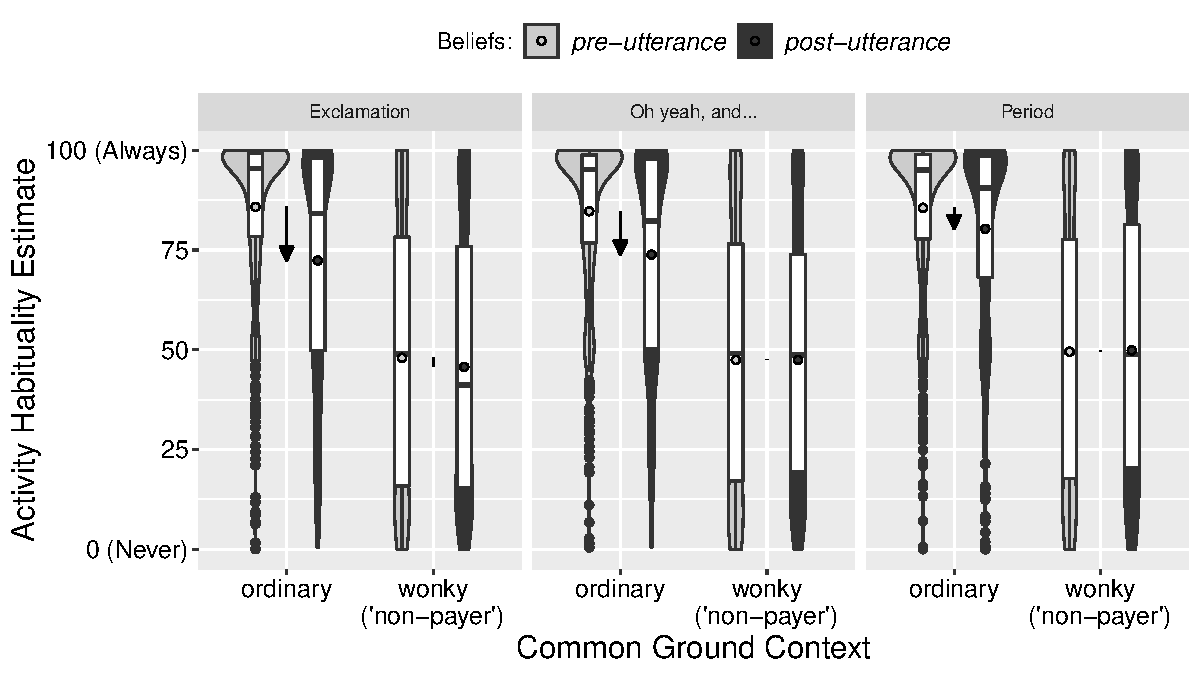
\includegraphics[width=\maxwidth]{figure/unnamed-chunk-66-1} \caption{\label{fig:expallhabitual}Experiments 1-3: \textit{conventionally habitual} (\textit{cashier-paying}) activity analysis.}\label{fig:unnamed-chunk-66}
\end{figure}


\end{knitrout}

The results are summarized in \ref{tab:expall}.  As predicted, the effect holds regardless of which relevance marker is used, and in fact there is no statistically significant difference between the two markers.  Further, the effect size of the common ground by belief measure interaction is significantly smaller in the absence of the markers; in other words, participants are significantly less likely to make a \textit{non-habituality} inference in the absence of a prosodic or discourse marker signaling relevance or intentionality\footnote{A similar cross-experiment analysis of the conventionally \textit{non-habitual} activities can be found in the supplementary materials: \url{https://osf.io/8fz4m/?view_only=ff5859d3f33b485d95254395f95a52dc}}.

The effect direction is consistent across experimental items, with by-item common ground by belief measure interaction effect sizes ranging from %
-5.06
 to %
-12.74
.  We again note here that this set of 3 experiments is a replication of a previously run set with somewhat less naturalistic stimuli, a full description of which can be found in the supplementary materials linked to in the previous paragraph. In addition, the `exclamation' experiment in that set is a further replication of a within-subects version (same stimuli), previously published as \citet{Kravtchenko2015}, where participants updated their own ratings after seeing the utterance.  We therefore argue that this is overall a robust and replicable effect.

This result clearly favors the "form sensitivity" hypothesis described in Section \ref{how-might-comprehenders-react-to-informational-redundancy} over a strong version of the "non-detachability" hypothesis (which might predict an effect of the same magnitude for all experiments).  We conclude that in the absence of a clear signal of utterance relevance or speaker intentionality, comprehenders are either less likely to attempt to resolve the violation, resolve it in a manner that is not reflected in our response measures, or do not detect the violation the first place. The first possibility is supported by observations that comprehenders approach speaker utterances \textit{charitably}, and may expend significant effort on interpreting them in a manner that is consistent with the speaker making cooperative conversational choices \citep{Davidson1974}. However, it is also possible that comprehenders are less `charitable' in general when presented with oddly phrased psycholinguistic stimuli in an artificial setting -- as well as less motivated on expending cognitive effort on calculating a non-obvious inference in a non-interactive environment, on the basis of an utterance that their attention is not otherwise drawn to.

Less charitable comprehenders, who may detect the redundancy but fail to in some way resolve it, may assume that the speaker is odd or not a particularly cooperative speaker, or perhaps that they are having production difficulties.  Another possibility is that they assume the speaker is in the process of planning a more informative utterance (where, for example, the description might serve as a temporal/causal anchor; see Example \ref{anchor}). Determining which strategies comprehenders do in fact resort to, and in which contexts, is left to future work. Finally, there is the possibility that, given the non-interactive experimental setting, comprehenders are processing the utterances at a relatively shallow level, and absent some (prosodic, discourse) indication that an utterance is somehow important, they do not expend effort on it \citep{Sanford2006}. To note, it has frequently been observed that comprehenders often do not make expected inferences in behavioral studies, for reasons that are not yet fully known \citep[cf.,][]{Noveck2003}. Determining whether this plays a role in our studies is left to future work, as is the question of whether similar or stronger effects can be observed in less artificial, and/or more interactive settings.

\subsection{Is the effect of habituality on pragmatic inferences gradient?}

Fig. \ref{fig:grad} plots the measured average activity habituality, with and without seeing the target utterance, for each item in each condition, for all three experiments. The diagonal dashed line demonstrates what the "no inference" hypothesis would predict: i.e., no effect of the utterance on belief change (\textit{pre-utterance} ratings mapping straightforwardly onto \textit{post-utterance} ratings). Points found above the line indicate that for those items, participants were more certain, for example, that \textit{John usually buys apples} when the story mentioned that "he got some apples." Points below the line indicate a \textit{non-habituality inference}: e.g., mentioning that "he paid the cashier" causes people to believe that \textit{John does not usually pay the cashier}.

\begin{knitrout}
\definecolor{shadecolor}{rgb}{0.969, 0.969, 0.969}\color{fgcolor}\begin{figure}
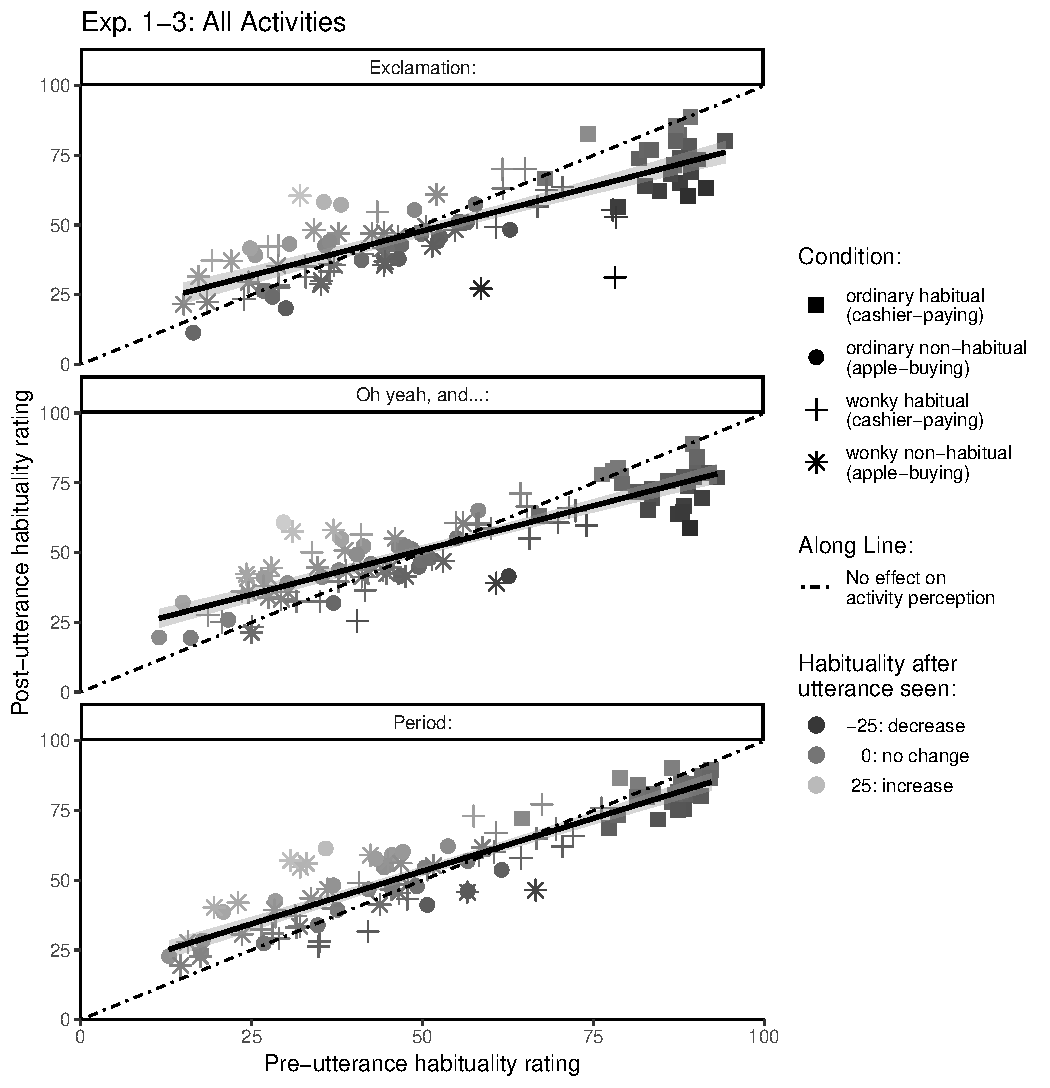
\includegraphics[width=\maxwidth]{figure/unnamed-chunk-69-1} \caption{\label{fig:grad}These plots show by-item belief change for all conditions of our three experiments. The dotted diagonal line represents the ``no inference'' hypothesis; i.e., what we would expect the data to look like if the critical utterance had no effect on habituality beliefs. The solid black line is a regression line with 95\% CIs across all conditions. The shading of the points represents the degree and direction of \textit{belief change}: negative/black indicates a \textit{non-habituality} inference; positive/light gray indicates a perception of increased habituality.}\label{fig:unnamed-chunk-69}
\end{figure}


\end{knitrout}

In Experiment 1 (exclamation mark), we see that for \textit{ordinary} common grounds, and \textit{conventionally-habitual} activities (e.g., \textit{paying the cashier} given an ordinary common ground), most data points fall below the line, indicating a non-habituality inference. Interestingly, we also see a gradual `trend' towards \textit{non-habituality} in the other three (non-redundant) conditions: items that are similar to \textit{ordinary habitual} items, in terms of pre-utterance habituality estimates, are more likely to trigger non-habituality inferences. In contrast, items with low pre-utterance habituality estimates show the opposite effect: i.e., if it's mentioned that an individual engaged in a particularly non-habitual activity, it leads comprehenders to believe that the individual is more likely to engage in that activity habitually. The same observations also hold for Experiment 2. 

In Experiment 3 (period), we again see a gradual effect of \textit{pre-utterance} beliefs regarding activity habituality on the likelihood of a \textit{non-habituality inference}, but this time the slope of the regression line is shifted upwards (Exp. 1: $\beta$=%
0.64
; Exp. 2: $\beta$=%
0.64
; Exp. 3: $\beta$=%
0.76
). We still see, however, that there is a gradient difference between highly expected vs. relatively expected events, in terms of likelihood of a non-habituality inference occurring.

Taken together, we can see in these figures that the exclamation mark and the `\textit{oh yeah...}' discourse marker, as signals of speaker effort and intentionality, make it more likely that non-habituality inferences will arise for \textit{ordinary} common ground, \textit{habitual} activity activity mentions. Furthermore, we can see that the effect of pre-utterance beliefs on non-habituality inferences is clearly gradient rather than binary: relatively more habitual activities, in all conditions, generally elicit larger \textit{non-habituality} inferences.

\section{General Discussion}\label{disc}

\subfile{sections/disc.tex}

\bibliography{prag}

\appendix

\pagebreak

\section{Replicated Work}\label{appendix}



\setcounter{secnumdepth}{5}

\subsection{Replicated experiments}

Here we present a previous iteration of this series of experiments, using the same design as that reported in the main body of the paper, but run on separate populations (as opposed to concurrently), and with a slightly different set of stimuli. We include these results here as evidence that the effects we report are robust, replicating closely despite being run on a different population, substantial revision of the stimuli to improve naturalness, addition of filler stimuli, and a larger amount of data being collected to improve power for all relevant comparisons.

\subsubsection{Methods}

\paragraph*{Participants}

1200 eligible participants (%
1242
 total), 400 per experiment, were recruited on Amazon Mechanical Turk, with the task only open to workers located in the US, and with an approval rating of $\geq$ 95\%. Participants who did not report their native language, or reported their native language as other than English, were excluded (%
42%
; %
3.38%
\%), with additional participants recruited to replace them.

\paragraph*{Materials}

The design was identical to that reported in the paper, aside from the inclusion of fillers, as each participant saw only 6 stimuli and no condition more than once, with all stimuli differing across multiple non-critical dimensions.  We therefore reasoned that there was little likelihood of learning the purpose of the experiment in the course of the task, and there was risk of increased task length/tedium decreasing the likelihood of participants reading passages closely enough to pick up on relatively subtle effects.

The stimuli in the replicated experiments were constructed to minimize variation in syntactic and information structure, as well as length, between stimuli.  However, this came at the cost of naturalness.  Here we present a stimulus example:


\ex.{\label{ex:oldstimulus}} \centering\textsc{Original Stimulus}

\begin{longtable}{p{0.435\textwidth}|p{0.435\textwidth}}
$[$1a$]$ John often \textit{goes to his local supermarket, as it's close by\textsubscript{ordinary}.} & $[$1b$]$ John often \textit{doesn't pay at the supermarket, as he's typically broke\textsubscript{wonky}.}\\
\hline
\multicolumn{2}{p{0.9\textwidth}}{$[$2$]$ Today he entered the apartment with his shopping bags flowing over. He ran into Susan, his best friend, and talked to her about his trip. Susan then wandered over to Peter, their roommate, who was in a different room.} \\
\hline
\multicolumn{2}{p{0.9\textwidth}}{$[$3$]$ Recently, he came home from the store with groceries.  When he came in, he saw his roommate Susan in the hallway, and started talking to her about his trip to the store.  As he went to the kitchen to put his groceries away, Susan went to the living room, where their roommate Peter was watching TV.} \\
\hline
\multicolumn{2}{p{0.9\textwidth}}{\centering$[$4$]$ She commented: ``John went shopping.} \\
\hline
$[$5a$]$ He \textbf{paid the \mbox{cashier\textsubscript{habitual}}}! & $[$5b$]$ He \textbf{got some apples\textsubscript{non-habitual}}!\\
\hline
\multicolumn{2}{p{0.9\textwidth}}{\centering$[$6$]$ I just saw him in the living room.''}
\end{longtable}
\addtocounter{table}{-1}


\paragraph*{Procedure}

The procedure was identical to that of the other experiments. 

\paragraph*{Measures}

The same response measures as in the other experiments were used to estimate \textit{pre-utterance beliefs} and \textit{post-utterance beliefs}. 

\subsubsection{Results}

As in the experiments reported in the main body of the paper, we modeled the difference between \textit{pre-utterance} and \textit{post-utterance} beliefs. \textit{Conventionally habitual} and conventionally \textit{non-habitual} activities were modeled separately. All binary factors were effect/sum coded, and the experiment factor was Helmert coded.

\paragraph*{\textit{Conventionally habitual} activities}$\quad$(`Paid the cashier')\\

The regression analysis showed a significant three-way interaction between discourse marker presence, common ground context, and belief measure: there was a significantly smaller \textit{atypicality} effect in Exp. 3 than in Experiments 1 and 2 ($\beta=$%
6.16%
, $p<$%
0.05%
), and no significant difference between Experiments 1 and 2 ($\beta=$%
0.42%
, $p=$%
0.89%
).

We used the maximal converging model, with by-subject random intercepts and slopes for common ground context (\textit{ordinary} / \textit{wonky}) and belief measure (\textit{pre-utterance} / \textit{post-utterance}), as well as by-item random intercepts and slopes for all factors. By-subject random slopes for the interaction were not included in the model, because we did not have any repeated measures for subjects for the interaction.  By-item random slopes for the interactions were not included in the model due to nonconvergence. A plot illustrating the higher-order experiment by common ground by belief measure interaction can be seen in Figure \ref{fig:oldexpallhabitual}.

%latex.default(coefs, file = "", title = "", table.env = TRUE,     booktabs = TRUE, caption = "Replicated Experiment 1-3: \\textit{conventionally habitual} (\\textit{cashier-paying}) activities analysis.",     label = "tab:oldexpall")%
\begin{table}[!tbp]
\caption{Replicated Experiment 1-3: \textit{conventionally habitual} (\textit{cashier-paying}) activities analysis.\label{tab:oldexpall}} 
\begin{center}
\begin{tabular}{lrrrl}
\toprule
\multicolumn{1}{l}{}&\multicolumn{1}{c}{$\beta$}&\multicolumn{1}{c}{SE($\beta$)}&\multicolumn{1}{c}{\textbf{t}}&\multicolumn{1}{c}{\textbf{p}}\tabularnewline
\midrule
Intercept&$ 61.22$&$2.11$&$29.01$&\textbf{\textless .001}\tabularnewline
`!' vs. `Oh yeah...'&$  1.30$&$1.02$&$ 1.28$&0.2\tabularnewline
`.' vs. Relevance Markers&$  4.34$&$0.88$&$ 4.92$&\textbf{\textless .001}\tabularnewline
Common Ground: Ordinary&$ 38.04$&$3.72$&$10.22$&\textbf{\textless .001}\tabularnewline
Belief: Post-utterance&$ -0.46$&$1.42$&$-0.32$&0.8\tabularnewline
`!' vs. `Oh yeah' * Common Ground&$ -0.87$&$1.82$&$-0.48$&0.6\tabularnewline
`.' vs. Relevance Markers * Common Ground&$  2.44$&$1.57$&$ 1.55$&0.1\tabularnewline
`!' vs. `Oh yeah' * Belief&$  0.61$&$1.76$&$ 0.35$&0.7\tabularnewline
`.' vs. Relevance Markers * Belief&$  6.68$&$1.52$&$ 4.39$&\textbf{\textless .001}\tabularnewline
Common Ground * Belief&$-12.66$&$1.27$&$-9.97$&\textbf{\textless .001}\tabularnewline
`!' vs. `Oh yeah' * CG * Belief&$  0.42$&$3.11$&$ 0.14$&0.9\tabularnewline
`.' vs. Relevance Markers * CG * Belief&$  6.16$&$2.69$&$ 2.29$&\textbf{\textless .05}\tabularnewline
\bottomrule
\end{tabular}\end{center}
\end{table}


\begin{figure}\begin{center}
\begin{knitrout}
\definecolor{shadecolor}{rgb}{0.969, 0.969, 0.969}\color{fgcolor}
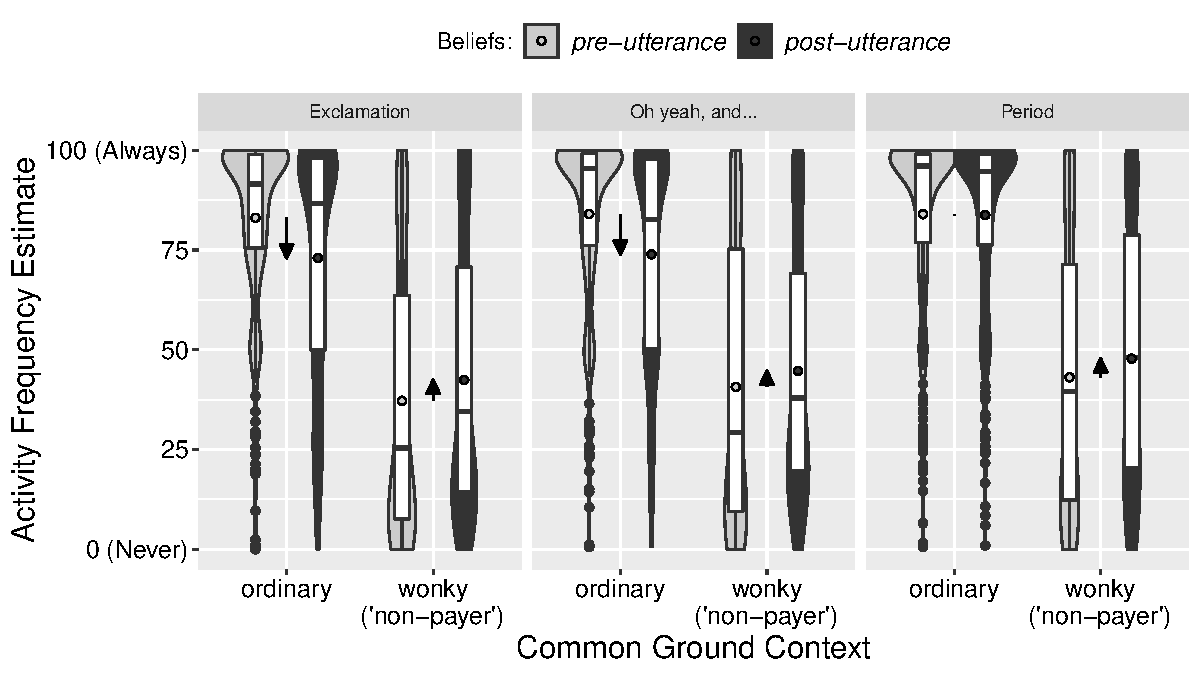
\includegraphics[width=\maxwidth]{figure/figure_1-1} 

\end{knitrout}
\end{center}
\caption{Replicated Experiments 1-3: \textit{conventionally habitual} (\textit{cashier-paying}) activities analysis.}
\label{fig:oldexpallhabitual}
\end{figure}

A similar analysis of the conventionally \textit{non-habitual} activities can be found in the next section of these materials.

\subsubsection{Discussion}

Overall, the results of these experiments were broadly replicated by those reported in the main body of the paper.  The only salient difference is that in the original iteration of Exp. 3, there was no measurable effect of informational redundancy on perceptions of activity typicality, while in the `new' Exp. 3, there was a significant, but diminished effect, as we had originally predicted.  The absence of a significant effect in the first iteration surprised us, and we attribute it to either chance (possibly due to fewer subjects run) or to increased prominence of the utterance in the revised stimuli.  To compare:

\ex. \textsc{Revised:} ``John just came back from the grocery store. \textbf{He paid the cashier}.''

\ex. \textsc{Original:} ``John went shopping. \textbf{He paid the cashier}. I just saw him in the living room.''

The utterance in question appears more discourse-prominent in the revised version of the stimuli, as it is utterance-final (i.e., we removed the last sentence), and in general competes with fewer adjacent utterances for attention.  We leave it to future work to definitively answer whether the minor change in utterance prominence does indeed eliminate the effect entirely.

\pagebreak

\subsection{Conventionally \textit{non-habitual} activities$\quad$(`Bought some apples')}

Here, we present the results of our cross-experiment analyses of \textit{non-habitual} activities.

\subsubsection{Experiments reported in paper}

We used the maximal converging model, with by-subject random intercepts and slopes for common ground context (\textit{ordinary} / \textit{wonky}) and belief measure (\textit{pre-utterance} / \textit{post-utterance}), by-item random intercepts and slopes for both factors and their interaction, and a by-item random slope for experiment. By-subject random slopes for the interaction were not included in the model due to lack of within-subject repeated measures in our data for the interaction. The random slope for the full by-item experiment by common ground by belief measure interaction was not included due to non-convergence.

The results are shown in Table \ref{tab:expallopt} and Figure \ref{fig:expallopt}.

%latex.default(coefs, file = "", title = "", table.env = TRUE,     booktabs = TRUE, caption = "Experiment 1-3: \\textit{conventionally non-habitual} (\\textit{apple-buying}) activities analysis.",     label = "tab:expallopt")%
\begin{table}[!tbp]
\caption{Experiment 1-3: \textit{conventionally non-habitual} (\textit{apple-buying}) activities analysis.\label{tab:expallopt}} 
\begin{center}
\begin{tabular}{lrrrl}
\toprule
\multicolumn{1}{l}{}&\multicolumn{1}{c}{$\beta$}&\multicolumn{1}{c}{SE($\beta$)}&\multicolumn{1}{c}{\textbf{t}}&\multicolumn{1}{c}{\textbf{p}}\tabularnewline
\midrule
Intercept&$41.18$&$1.89$&$21.84$&\textbf{\textless .001}\tabularnewline
`!' vs. `Oh yeah...'&$ 0.84$&$0.72$&$ 1.17$&0.2\tabularnewline
`.' vs. Relevance Markers&$ 1.50$&$0.62$&$ 2.41$&\textbf{\textless .05}\tabularnewline
Common Ground: Ordinary&$ 2.00$&$1.97$&$ 1.02$&0.3\tabularnewline
Belief: Post-utterance&$ 4.51$&$1.70$&$ 2.65$&\textbf{\textless .05}\tabularnewline
`!' vs. `Oh yeah' * Common Ground&$-2.11$&$1.05$&$-2.02$&\textbf{\textless .05}\tabularnewline
`.' vs. Relevance Markers * Common Ground&$ 0.34$&$0.91$&$ 0.38$&0.7\tabularnewline
`!' vs. `Oh yeah' * Belief&$ 3.71$&$1.11$&$ 3.34$&\textbf{\textless .001}\tabularnewline
`.' vs. Relevance Markers * Belief&$ 3.76$&$0.96$&$ 3.90$&\textbf{\textless .001}\tabularnewline
Common Ground * Belief&$-0.73$&$1.43$&$-0.51$&0.6\tabularnewline
`!' vs. `Oh yeah' * CG * Belief&$-1.34$&$2.07$&$-0.65$&0.5\tabularnewline
`.' vs. Relevance Markers * CG * Belief&$-0.64$&$1.79$&$-0.35$&0.7\tabularnewline
\bottomrule
\end{tabular}\end{center}
\end{table}


\begin{figure}\begin{center}
\begin{knitrout}
\definecolor{shadecolor}{rgb}{0.969, 0.969, 0.969}\color{fgcolor}
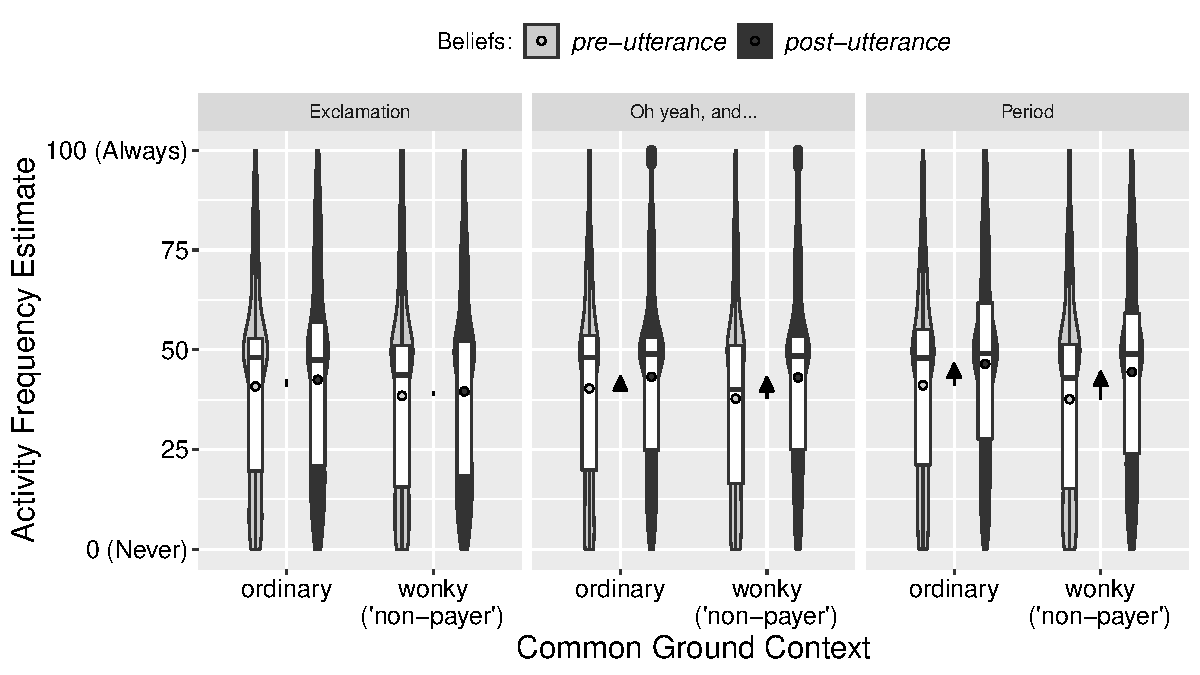
\includegraphics[width=\maxwidth]{figure/suppfig1-1} 

\end{knitrout}
\end{center}
\caption{Experiment 1-3: \textit{conventionally non-habitual} (\textit{apple-buying}) activities analysis.}
\label{fig:expallopt}
\end{figure}

\subsubsection{Replicated experiments}

We used the maximal converging model, with by-subject random intercepts and slopes for common ground context (\textit{ordinary} / \textit{wonky}) and belief measure (\textit{pre-utterance} / \textit{post-utterance}), and by-item random intercepts and slopes for both factors and their interaction. By-subject random slopes for the interaction were not included in the model due to lack of within-subject repeated measures in our data for the interaction. The by-item random slope experiment was not included due to non-convergence.

The results are shown in Table \ref{tab:oldexpallopt} and Figure \ref{fig:oldexpallopt}.

%latex.default(coefs, file = "", title = "", table.env = TRUE,     booktabs = TRUE, caption = "Replicated Experiments 1-3: conventionally \\textit{non-habitual} (\\textit{apple-buying}) activities analysis.",     label = "tab:oldexpallopt")%
\begin{table}[!tbp]
\caption{Replicated Experiments 1-3: conventionally \textit{non-habitual} (\textit{apple-buying}) activities analysis.\label{tab:oldexpallopt}} 
\begin{center}
\begin{tabular}{lrrrl}
\toprule
\multicolumn{1}{l}{}&\multicolumn{1}{c}{$\beta$}&\multicolumn{1}{c}{SE($\beta$)}&\multicolumn{1}{c}{\textbf{t}}&\multicolumn{1}{c}{\textbf{p}}\tabularnewline
\midrule
Intercept&$39.80$&$2.47$&$16.09$&\textbf{\textless .001}\tabularnewline
`!' vs. `Oh yeah...'&$ 2.25$&$1.01$&$ 2.22$&\textbf{\textless .05}\tabularnewline
`.' vs. Relevance Markers&$ 2.33$&$1.02$&$ 2.28$&\textbf{\textless .05}\tabularnewline
Common Ground: Ordinary&$ 2.98$&$2.01$&$ 1.49$&0.2\tabularnewline
Belief: Post-utterance&$ 6.20$&$1.98$&$ 3.14$&\textbf{\textless .01}\tabularnewline
`!' vs. `Oh yeah' * Common Ground&$-0.02$&$1.40$&$-0.02$&1\tabularnewline
`.' vs. Relevance Markers * Common Ground&$ 1.05$&$1.22$&$ 0.87$&0.4\tabularnewline
`!' vs. `Oh yeah' * Belief&$ 4.37$&$1.53$&$ 2.85$&\textbf{\textless .01}\tabularnewline
`.' vs. Relevance Markers * Belief&$ 5.52$&$1.33$&$ 4.15$&\textbf{\textless .001}\tabularnewline
Common Ground * Belief&$-4.65$&$1.14$&$-4.08$&\textbf{\textless .001}\tabularnewline
`!' vs. `Oh yeah' * CG * Belief&$-3.38$&$2.80$&$-1.21$&0.2\tabularnewline
`.' vs. Relevance Markers * CG * Belief&$-4.28$&$2.43$&$-1.76$&0.1\tabularnewline
\bottomrule
\end{tabular}\end{center}
\end{table}


\begin{figure}\begin{center}
\begin{knitrout}
\definecolor{shadecolor}{rgb}{0.969, 0.969, 0.969}\color{fgcolor}
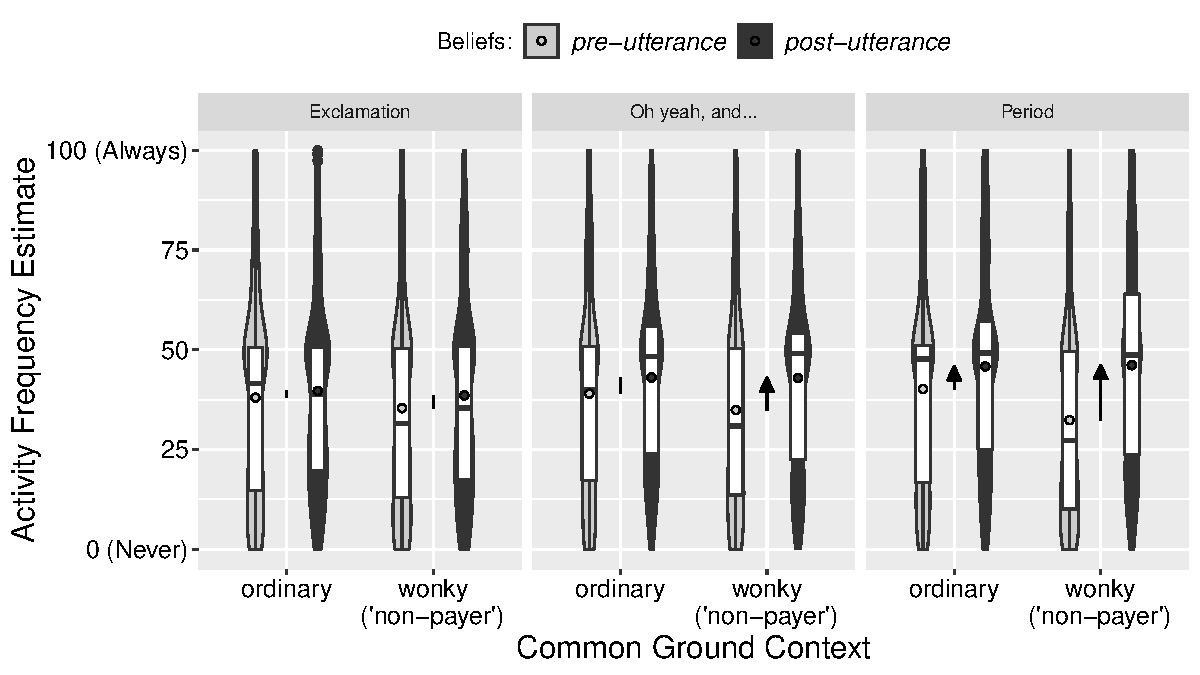
\includegraphics[width=\maxwidth]{figure/suppfig2-1} 

\end{knitrout}
\end{center}
\caption{Replicated Experiments 1-3: \textit{conventionally non-habitual} (\textit{apple-buying}) activities analysis.}
\label{fig:oldexpallopt}
\end{figure}

\pagebreak

\section{Experimental Stimuli}\label{stimuli}

\subfile{sections/stimuli.tex}

\pagebreak

\section{Power Analysis}\label{power}

\begin{knitrout}\small
\definecolor{shadecolor}{rgb}{0.969, 0.969, 0.969}\color{fgcolor}\begin{kframe}
\begin{alltt}
\hlcom{# Power by simulation for a normally distributed}
\hlcom{# continuous outcome with subjects, items, and residual}
\hlcom{# variability}

\hlcom{# Population parameters mu: underlying mean of the}
\hlcom{# outcome in the reference group betaN: effect size of}
\hlcom{# predictor or interaction sdItem: sd of random effect}
\hlcom{# at the item level sdSubject: sd of random effect at}
\hlcom{# the subject level sdResid: sd of residual error}

\hlcom{# Design parameters nSubjects: number of subjects in}
\hlcom{# simulation nIterations: number of iterations in}
\hlcom{# simulation}

\hlstd{fnPower} \hlkwb{<-} \hlkwa{function}\hlstd{(}\hlkwc{mu}\hlstd{,} \hlkwc{beta1}\hlstd{,} \hlkwc{beta2}\hlstd{,} \hlkwc{beta3}\hlstd{,} \hlkwc{beta4}\hlstd{,} \hlkwc{beta5}\hlstd{,}
    \hlkwc{beta6}\hlstd{,} \hlkwc{beta7}\hlstd{,} \hlkwc{beta8}\hlstd{,} \hlkwc{beta9}\hlstd{,} \hlkwc{beta10}\hlstd{,} \hlkwc{beta11}\hlstd{,} \hlkwc{sdItem}\hlstd{,}
    \hlkwc{sdSubject}\hlstd{,} \hlkwc{sdResid}\hlstd{,} \hlkwc{nSubjects}\hlstd{,} \hlkwc{nIterations}\hlstd{,} \hlkwc{dots} \hlstd{=} \hlnum{TRUE}\hlstd{) \{}
    \hlstd{start.time} \hlkwb{<-} \hlkwd{Sys.time}\hlstd{()}
    \hlstd{progress} \hlkwb{<-} \hlstr{") \textbackslash{}n----|--- 1 ---|--- 2 ---|--- 3 ---|--- 4 ---| --- 5 \textbackslash{}n"}
    \hlkwa{if} \hlstd{(dots)}
        \hlkwd{cat}\hlstd{(}\hlstr{"Simulations ("}\hlstd{, nIterations, progress,} \hlkwc{sep} \hlstd{=} \hlstr{""}\hlstd{)}
    \hlcom{# objects to store pvalue, beta, and standard error from}
    \hlcom{# each iteration of simulation}
    \hlstd{pVals} \hlkwb{<-} \hlstd{betaVals} \hlkwb{<-} \hlstd{seVals} \hlkwb{<-} \hlkwd{matrix}\hlstd{(}\hlnum{NA}\hlstd{,} \hlkwc{nrow} \hlstd{= nIterations,}
        \hlkwc{ncol} \hlstd{=} \hlnum{11}\hlstd{)}
    \hlcom{# build design matrices}
    \hlstd{m} \hlkwb{<-} \hlkwd{matrix}\hlstd{(}\hlnum{NA}\hlstd{,} \hlkwc{nrow} \hlstd{= nSubjects} \hlopt{*} \hlnum{4}\hlstd{,} \hlkwc{ncol} \hlstd{=} \hlnum{7}\hlstd{)}
    \hlkwd{colnames}\hlstd{(m)} \hlkwb{<-} \hlkwd{c}\hlstd{(}\hlstr{"worker"}\hlstd{,} \hlstr{"exp.alike"}\hlstd{,} \hlstr{"exp.diff"}\hlstd{,}
        \hlstr{"story"}\hlstd{,} \hlstr{"condition"}\hlstd{,} \hlstr{"context"}\hlstd{,} \hlstr{"slider"}\hlstd{)}
    \hlstd{m[,} \hlnum{1}\hlstd{]} \hlkwb{<-} \hlkwd{rep}\hlstd{(}\hlnum{1}\hlopt{:}\hlstd{nSubjects,} \hlkwc{each} \hlstd{=} \hlnum{4}\hlstd{)}
    \hlstd{m[,} \hlnum{2}\hlstd{]} \hlkwb{<-} \hlkwd{rep}\hlstd{(}\hlkwd{c}\hlstd{(}\hlopt{-}\hlnum{0.5}\hlstd{,} \hlnum{0.5}\hlstd{,} \hlnum{0}\hlstd{),} \hlkwc{each} \hlstd{=} \hlnum{4}\hlstd{,} \hlkwc{length.out} \hlstd{=} \hlkwd{length}\hlstd{(m[,}
        \hlnum{2}\hlstd{]))}
    \hlstd{m[,} \hlnum{3}\hlstd{]} \hlkwb{<-} \hlkwd{rep}\hlstd{(}\hlkwd{c}\hlstd{(}\hlopt{-}\hlnum{0.3333333}\hlstd{,} \hlopt{-}\hlnum{0.3333333}\hlstd{,} \hlnum{0.6666667}\hlstd{),}
        \hlkwc{each} \hlstd{=} \hlnum{4}\hlstd{,} \hlkwc{length.out} \hlstd{=} \hlkwd{length}\hlstd{(m[,} \hlnum{3}\hlstd{]))}
    \hlstd{i} \hlkwb{<-} \hlnum{1}
    \hlkwa{while} \hlstd{(i} \hlopt{<} \hlstd{(}\hlkwd{length}\hlstd{(m[,} \hlnum{4}\hlstd{]))) \{}
        \hlstd{m[i}\hlopt{:}\hlstd{(i} \hlopt{+} \hlnum{3}\hlstd{),} \hlnum{4}\hlstd{]} \hlkwb{<-} \hlkwd{sample}\hlstd{(}\hlnum{1}\hlopt{:}\hlnum{24}\hlstd{,} \hlkwc{size} \hlstd{=} \hlnum{4}\hlstd{,} \hlkwc{replace} \hlstd{=} \hlnum{FALSE}\hlstd{)}
        \hlstd{i} \hlkwb{<-} \hlstd{i} \hlopt{+} \hlnum{4}
    \hlstd{\}}
    \hlstd{m[,} \hlnum{5}\hlstd{]} \hlkwb{<-} \hlkwd{rep}\hlstd{(}\hlkwd{c}\hlstd{(}\hlopt{-}\hlnum{0.5}\hlstd{,} \hlnum{0.5}\hlstd{))}
    \hlstd{m[,} \hlnum{6}\hlstd{]} \hlkwb{<-} \hlkwd{rep}\hlstd{(}\hlkwd{c}\hlstd{(}\hlopt{-}\hlnum{0.5}\hlstd{,} \hlnum{0.5}\hlstd{),} \hlkwc{each} \hlstd{=} \hlnum{2}\hlstd{)}
    \hlcom{# i <- 1 # (when testing for-loop)}
    \hlkwa{for} \hlstd{(i} \hlkwa{in} \hlnum{1}\hlopt{:}\hlstd{nIterations) \{}

        \hlcom{# draw random effects}
        \hlstd{itemRE} \hlkwb{<-} \hlkwd{rnorm}\hlstd{(}\hlnum{24}\hlstd{,} \hlnum{0}\hlstd{, sdItem)}
        \hlstd{subjRE} \hlkwb{<-} \hlkwd{rnorm}\hlstd{(nSubjects,} \hlnum{0}\hlstd{, sdSubject)}
        \hlstd{residRE} \hlkwb{<-} \hlkwd{rnorm}\hlstd{(}\hlkwd{nrow}\hlstd{(m),} \hlnum{0}\hlstd{, sdResid)}

        \hlcom{# create outcome}
        \hlstd{y} \hlkwb{<-} \hlstd{mu} \hlopt{+} \hlstd{beta1} \hlopt{*} \hlstd{m[,} \hlnum{2}\hlstd{]} \hlopt{+} \hlstd{beta2} \hlopt{*} \hlstd{m[,} \hlnum{3}\hlstd{]} \hlopt{+} \hlstd{beta3} \hlopt{*}
            \hlstd{m[,} \hlnum{6}\hlstd{]} \hlopt{+} \hlstd{beta4} \hlopt{*} \hlstd{m[,} \hlnum{5}\hlstd{]} \hlopt{+} \hlstd{beta5} \hlopt{*} \hlstd{m[,} \hlnum{2}\hlstd{]} \hlopt{*} \hlstd{m[,}
            \hlnum{6}\hlstd{]} \hlopt{+} \hlstd{beta6} \hlopt{*} \hlstd{m[,} \hlnum{3}\hlstd{]} \hlopt{*} \hlstd{m[,} \hlnum{6}\hlstd{]} \hlopt{+} \hlstd{beta7} \hlopt{*} \hlstd{m[,} \hlnum{2}\hlstd{]} \hlopt{*}
            \hlstd{m[,} \hlnum{5}\hlstd{]} \hlopt{+} \hlstd{beta8} \hlopt{*} \hlstd{m[,} \hlnum{3}\hlstd{]} \hlopt{*} \hlstd{m[,} \hlnum{5}\hlstd{]} \hlopt{+} \hlstd{beta9} \hlopt{*} \hlstd{m[,}
            \hlnum{6}\hlstd{]} \hlopt{*} \hlstd{m[,} \hlnum{5}\hlstd{]} \hlopt{+} \hlstd{beta10} \hlopt{*} \hlstd{m[,} \hlnum{2}\hlstd{]} \hlopt{*} \hlstd{m[,} \hlnum{6}\hlstd{]} \hlopt{*} \hlstd{m[,}
            \hlnum{5}\hlstd{]} \hlopt{+} \hlstd{beta11} \hlopt{*} \hlstd{m[,} \hlnum{3}\hlstd{]} \hlopt{*} \hlstd{m[,} \hlnum{6}\hlstd{]} \hlopt{*} \hlstd{m[,} \hlnum{5}\hlstd{]} \hlopt{+} \hlstd{itemRE[m[,}
            \hlnum{4}\hlstd{]]} \hlopt{+} \hlstd{subjRE[m[,} \hlnum{1}\hlstd{]]} \hlopt{+} \hlstd{residRE}
        \hlstd{m[,} \hlnum{7}\hlstd{]} \hlkwb{<-} \hlstd{y}
        \hlstd{dm} \hlkwb{<-} \hlkwd{as.data.frame}\hlstd{(m)}
        \hlstd{dm}\hlopt{$}\hlstd{worker} \hlkwb{<-} \hlkwd{as.factor}\hlstd{(dm}\hlopt{$}\hlstd{worker)}
        \hlstd{dm}\hlopt{$}\hlstd{story} \hlkwb{<-} \hlkwd{as.factor}\hlstd{(dm}\hlopt{$}\hlstd{story)}
        \hlcom{# fit model, store p-value, beta and standard error}
        \hlstd{o} \hlkwb{<-} \hlkwd{lmer}\hlstd{(slider} \hlopt{~} \hlstd{exp.alike} \hlopt{+} \hlstd{exp.diff} \hlopt{+} \hlstd{context} \hlopt{+}
            \hlstd{condition} \hlopt{+} \hlstd{exp.alike}\hlopt{:}\hlstd{context} \hlopt{+} \hlstd{exp.diff}\hlopt{:}\hlstd{context} \hlopt{+}
            \hlstd{exp.alike}\hlopt{:}\hlstd{condition} \hlopt{+} \hlstd{exp.diff}\hlopt{:}\hlstd{condition} \hlopt{+} \hlstd{context}\hlopt{:}\hlstd{condition} \hlopt{+}
            \hlstd{exp.alike}\hlopt{:}\hlstd{context}\hlopt{:}\hlstd{condition} \hlopt{+} \hlstd{exp.diff}\hlopt{:}\hlstd{context}\hlopt{:}\hlstd{condition} \hlopt{+}
            \hlstd{(}\hlnum{1} \hlopt{|} \hlstd{story)} \hlopt{+} \hlstd{(}\hlnum{1} \hlopt{|} \hlstd{worker), dm)}
        \hlstd{pVals[i, ]} \hlkwb{<-} \hlkwd{coef}\hlstd{(}\hlkwd{summary}\hlstd{(o))[}\hlnum{2}\hlopt{:}\hlnum{12}\hlstd{,} \hlnum{5}\hlstd{]}
        \hlstd{betaVals[i, ]} \hlkwb{<-} \hlkwd{coef}\hlstd{(}\hlkwd{summary}\hlstd{(o))[}\hlnum{2}\hlopt{:}\hlnum{12}\hlstd{,} \hlnum{1}\hlstd{]}
        \hlstd{seVals[i, ]} \hlkwb{<-} \hlkwd{coef}\hlstd{(}\hlkwd{summary}\hlstd{(o))[}\hlnum{2}\hlopt{:}\hlnum{12}\hlstd{,} \hlnum{2}\hlstd{]}

        \hlkwa{if} \hlstd{(dots)}
            \hlkwd{cat}\hlstd{(}\hlstr{"."}\hlstd{,} \hlkwc{sep} \hlstd{=} \hlstr{""}\hlstd{)}
        \hlkwa{if} \hlstd{(dots} \hlopt{&&} \hlstd{i}\hlopt\hlnum{50} \hlopt{==} \hlnum{0}\hlstd{)}
            \hlkwd{cat}\hlstd{(i,} \hlstr{"\textbackslash{}n"}\hlstd{)}

    \hlstd{\}}

    \hlkwa{if} \hlstd{(dots)}
        \hlkwd{cat}\hlstd{(}\hlstr{"\textbackslash{}nSimulation Run Time:"}\hlstd{,} \hlkwd{round}\hlstd{(}\hlkwd{difftime}\hlstd{(}\hlkwd{Sys.time}\hlstd{(),}
            \hlstd{start.time,} \hlkwc{units} \hlstd{=} \hlstr{"hours"}\hlstd{),} \hlnum{3}\hlstd{),} \hlstr{" Hours \textbackslash{}n"}\hlstd{)}

    \hlcom{# calculate power}
    \hlstd{powerOut} \hlkwb{<-} \hlkwd{apply}\hlstd{(pVals,} \hlnum{2}\hlstd{,} \hlkwa{function}\hlstd{(}\hlkwc{x}\hlstd{)} \hlkwd{length}\hlstd{(x[x} \hlopt{<}
        \hlnum{0.05}\hlstd{])}\hlopt{/}\hlkwd{length}\hlstd{(x))}
    \hlkwd{return}\hlstd{(}\hlkwd{list}\hlstd{(}\hlkwc{power} \hlstd{= powerOut,} \hlkwc{p} \hlstd{= pVals,} \hlkwc{beta} \hlstd{= betaVals,}
        \hlkwc{se} \hlstd{= seVals))}
\hlstd{\}}


\hlcom{# calibrate by setting betas = 0; histograms should all}
\hlcom{# look level, with about 5% of results significant by}
\hlcom{# chance}
\hlstd{outCalibrate} \hlkwb{<-} \hlkwd{fnPower}\hlstd{(}\hlkwc{mu} \hlstd{=} \hlnum{61.0444}\hlstd{,} \hlkwc{beta1} \hlstd{=} \hlnum{0}\hlstd{,} \hlkwc{beta2} \hlstd{=} \hlnum{0}\hlstd{,}
    \hlkwc{beta3} \hlstd{=} \hlnum{0}\hlstd{,} \hlkwc{beta4} \hlstd{=} \hlnum{0}\hlstd{,} \hlkwc{beta5} \hlstd{=} \hlnum{0}\hlstd{,} \hlkwc{beta6} \hlstd{=} \hlnum{0}\hlstd{,} \hlkwc{beta7} \hlstd{=} \hlnum{0}\hlstd{,}
    \hlkwc{beta8} \hlstd{=} \hlnum{0}\hlstd{,} \hlkwc{beta9} \hlstd{=} \hlnum{0}\hlstd{,} \hlkwc{beta10} \hlstd{=} \hlnum{0}\hlstd{,} \hlkwc{beta11} \hlstd{=} \hlnum{0}\hlstd{,} \hlkwc{sdItem} \hlstd{=} \hlnum{10.138}\hlstd{,}
    \hlkwc{sdSubject} \hlstd{=} \hlnum{9.285}\hlstd{,} \hlkwc{sdResid} \hlstd{=} \hlnum{21.839}\hlstd{,} \hlkwc{nSubjects} \hlstd{=} \hlnum{1200}\hlstd{,}
    \hlkwc{nIterations} \hlstd{=} \hlnum{10000}\hlstd{,} \hlkwc{dots} \hlstd{=} \hlnum{TRUE}\hlstd{)}
\hlstd{outCalibrate}\hlopt{$}\hlstd{power}
\hlkwd{hist}\hlstd{(outCalibrate}\hlopt{$}\hlstd{p[,} \hlnum{1}\hlstd{],} \hlkwc{main} \hlstd{=} \hlstr{"beta1"}\hlstd{,} \hlkwc{xlab} \hlstd{=} \hlstr{"p value"}\hlstd{)}
\hlkwd{hist}\hlstd{(outCalibrate}\hlopt{$}\hlstd{p[,} \hlnum{2}\hlstd{],} \hlkwc{main} \hlstd{=} \hlstr{"beta2"}\hlstd{,} \hlkwc{xlab} \hlstd{=} \hlstr{"p value"}\hlstd{)}
\hlkwd{hist}\hlstd{(outCalibrate}\hlopt{$}\hlstd{p[,} \hlnum{3}\hlstd{],} \hlkwc{main} \hlstd{=} \hlstr{"beta3"}\hlstd{,} \hlkwc{xlab} \hlstd{=} \hlstr{"p value"}\hlstd{)}
\hlkwd{hist}\hlstd{(outCalibrate}\hlopt{$}\hlstd{p[,} \hlnum{4}\hlstd{],} \hlkwc{main} \hlstd{=} \hlstr{"beta4"}\hlstd{,} \hlkwc{xlab} \hlstd{=} \hlstr{"p value"}\hlstd{)}
\hlkwd{hist}\hlstd{(outCalibrate}\hlopt{$}\hlstd{p[,} \hlnum{5}\hlstd{],} \hlkwc{main} \hlstd{=} \hlstr{"beta5"}\hlstd{,} \hlkwc{xlab} \hlstd{=} \hlstr{"p value"}\hlstd{)}
\hlkwd{hist}\hlstd{(outCalibrate}\hlopt{$}\hlstd{p[,} \hlnum{6}\hlstd{],} \hlkwc{main} \hlstd{=} \hlstr{"beta6"}\hlstd{,} \hlkwc{xlab} \hlstd{=} \hlstr{"p value"}\hlstd{)}
\hlkwd{hist}\hlstd{(outCalibrate}\hlopt{$}\hlstd{p[,} \hlnum{7}\hlstd{],} \hlkwc{main} \hlstd{=} \hlstr{"beta7"}\hlstd{,} \hlkwc{xlab} \hlstd{=} \hlstr{"p value"}\hlstd{)}
\hlkwd{hist}\hlstd{(outCalibrate}\hlopt{$}\hlstd{p[,} \hlnum{8}\hlstd{],} \hlkwc{main} \hlstd{=} \hlstr{"beta8"}\hlstd{,} \hlkwc{xlab} \hlstd{=} \hlstr{"p value"}\hlstd{)}
\hlkwd{hist}\hlstd{(outCalibrate}\hlopt{$}\hlstd{p[,} \hlnum{9}\hlstd{],} \hlkwc{main} \hlstd{=} \hlstr{"beta9"}\hlstd{,} \hlkwc{xlab} \hlstd{=} \hlstr{"p value"}\hlstd{)}
\hlkwd{hist}\hlstd{(outCalibrate}\hlopt{$}\hlstd{p[,} \hlnum{10}\hlstd{],} \hlkwc{main} \hlstd{=} \hlstr{"beta10"}\hlstd{,} \hlkwc{xlab} \hlstd{=} \hlstr{"p value"}\hlstd{)}
\hlkwd{hist}\hlstd{(outCalibrate}\hlopt{$}\hlstd{p[,} \hlnum{11}\hlstd{],} \hlkwc{main} \hlstd{=} \hlstr{"beta11"}\hlstd{,} \hlkwc{xlab} \hlstd{=} \hlstr{"p value"}\hlstd{)}

\hlstd{nSubjects} \hlkwb{<-} \hlkwd{seq}\hlstd{(}\hlnum{1200}\hlstd{,} \hlnum{2400}\hlstd{,} \hlnum{100}\hlstd{)}

\hlstd{st} \hlkwb{<-} \hlkwd{c}\hlstd{()}
\hlkwa{for} \hlstd{(i} \hlkwa{in} \hlnum{1}\hlopt{:}\hlkwd{length}\hlstd{(nSubjects)) \{}
    \hlstd{st[[}\hlkwd{paste}\hlstd{(}\hlstr{"subj"}\hlstd{, nSubjects[i])]]} \hlkwb{<-} \hlkwd{fnPower}\hlstd{(}\hlkwc{mu} \hlstd{=} \hlnum{61.2216}\hlstd{,}
        \hlkwc{beta1} \hlstd{=} \hlnum{1.3018}\hlstd{,} \hlkwc{beta2} \hlstd{=} \hlnum{4.3355}\hlstd{,} \hlkwc{beta3} \hlstd{=} \hlnum{38.0383}\hlstd{,}
        \hlkwc{beta4} \hlstd{=} \hlopt{-}\hlnum{0.4559}\hlstd{,} \hlkwc{beta5} \hlstd{=} \hlopt{-}\hlnum{0.8669}\hlstd{,} \hlkwc{beta6} \hlstd{=} \hlnum{2.4416}\hlstd{,}
        \hlkwc{beta7} \hlstd{=} \hlnum{0.6141}\hlstd{,} \hlkwc{beta8} \hlstd{=} \hlnum{6.6776}\hlstd{,} \hlkwc{beta9} \hlstd{=} \hlopt{-}\hlnum{12.6572}\hlstd{,}
        \hlkwc{beta10} \hlstd{=} \hlnum{0.4207}\hlstd{,} \hlkwc{beta11} \hlstd{=} \hlnum{6.1601}\hlstd{,} \hlkwc{sdItem} \hlstd{=} \hlnum{10.138}\hlstd{,}
        \hlkwc{sdSubject} \hlstd{=} \hlnum{9.285}\hlstd{,} \hlkwc{sdResid} \hlstd{=} \hlnum{21.839}\hlstd{,} \hlkwc{nSubjects} \hlstd{= nSubjects[i],}
        \hlkwc{nIterations} \hlstd{=} \hlnum{1000}\hlstd{,} \hlkwc{dots} \hlstd{=} \hlnum{TRUE}\hlstd{)}
\hlstd{\}}
\end{alltt}
\end{kframe}
\end{knitrout}




\subsection{Plot}

Figure \ref{fig:power} shows a plot of the power curves for the critical common ground by belief measure interaction, a comparison of that effect across Experiments 1 and 2, and another comparison across Experiment 3 and Experiments 1/2 (as a group).  We expect a robustly replicable common ground by belief measure interaction (power $= 1.00$ at all sample sizes), no significant difference between Experiments 1 and 2 (power $\leq 0.1$ at all sample sizes), and a significant difference between Experiment 3 and Experiments 1/2 (power $\geq$ 0.85 at a sample size of 2100 or more).

\begin{figure}\begin{center}
\begin{knitrout}
\definecolor{shadecolor}{rgb}{0.969, 0.969, 0.969}\color{fgcolor}
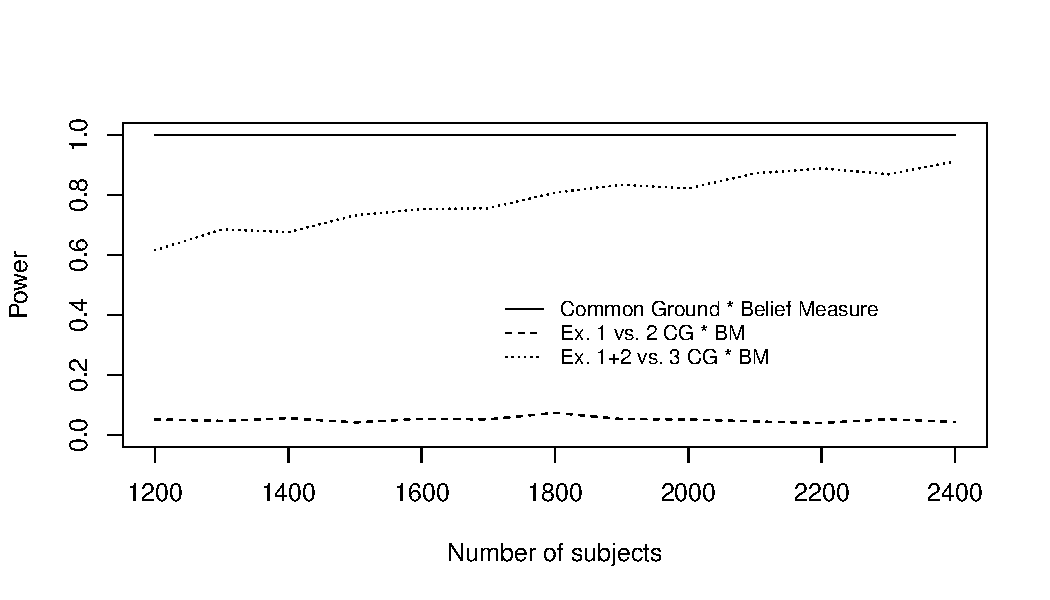
\includegraphics[width=\maxwidth]{figure/powerfig-1} 

\end{knitrout}
\end{center}
\caption{Power curves for effects of interest}
\label{fig:power}
\end{figure}


\end{document}
